%% abtex2-modelo-trabalho-academico.tex, v-1.9.2 laurocesar
%% Copyright 2012-2014 by abnTeX2 group at http://abntex2.googlecode.com/ 
%%
%% This work may be distributed and/or modified under the
%% conditions of the LaTeX Project Public License, either version 1.3
%% of this license or (at your option) any later version.
%% The latest version of this license is in
%%   http://www.latex-project.org/lppl.txt
%% and version 1.3 or later is part of all distributions of LaTeX
%% version 2005/12/01 or later.
%%
%% This work has the LPPL maintenance status `maintained'.
%% 
%% The Current Maintainer of this work is the abnTeX2 team, led
%% by Lauro César Araujo. Further information are available on 
%% http://abntex2.googlecode.com/
%%
%% This work consists of the files abntex2-modelo-trabalho-academico.tex,
%% abntex2-modelo-include-comandos and abntex2-modelo-references.bib
%%

% ------------------------------------------------------------------------
% ------------------------------------------------------------------------
% abnTeX2: Modelo de Trabalho Academico (tese de doutorado, dissertacao de
% mestrado e trabalhos monograficos em geral) em conformidade com 
% ABNT NBR 14724:2011: Informacao e documentacao - Trabalhos academicos -
% Apresentacao
% ------------------------------------------------------------------------
% ------------------------------------------------------------------------

%-------------------------------------------------------------------------
% Modelo adaptado especificamente para o contexto do PPgSI-EACH-USP por 
% Marcelo Fantinato, com auxílio dos Professores Norton T. Roman, Helton
% H. Bíscaro, e Sarajane M. Peres, em 2015, com muitos agradecimentos aos 
% criadores da classe e do modelo base.
%-------------------------------------------------------------------------

\documentclass[
	% -- opções da classe memoir --
	12pt,				% tamanho da fonte
	% openright,			% capítulos começam em pág ímpar (insere página vazia caso preciso)
	oneside,			% para impressão apenas no anverso (apenas frente). Oposto a twoside
	a4paper,			% tamanho do papel. 
	% -- opções da classe abntex2 --
	%chapter=TITLE,		% títulos de capítulos convertidos em letras maiúsculas
	%section=TITLE,		% títulos de seções convertidos em letras maiúsculas
	%subsection=TITLE,	% títulos de subseções convertidos em letras maiúsculas
	%subsubsection=TITLE,% títulos de subsubseções convertidos em letras maiúsculas
	% -- opções do pacote babel --
	english,			% idioma adicional para hifenização
	%french,				% idioma adicional para hifenização
	%spanish,			% idioma adicional para hifenização
	brazil				% o último idioma é o principal do documento
	]{abntex2ppgsi}

%Altera o espacamento entre equações
\setlength{\jot}{7pt}


%\newcommand{\@autor}{Adilson Lopes Khouri, 2015}
\def \varAutorData {Adilson Lopes Khouri, 2016}
% ---
% Pacotes básicos 
% ---
\usepackage[utf8]{inputenc}		% Codificacao do documento (conversão automática dos acentos)
\usepackage{lastpage}			% Usado pela Ficha catalográfica
\usepackage{indentfirst}		% Indenta o primeiro parágrafo de cada seção.
\usepackage{color}				% Controle das cores
\usepackage{graphicx}			% Inclusão de gráficos

\usepackage{microtype} 			% para melhorias de justificação
\DisableLigatures{encoding = *, family = *} %Remove ligaduras, tornando o texto bonito

\usepackage{pdfpages}     		%para incluir pdf
\usepackage{algorithm}			%para ilustrações do tipo algoritmo
\usepackage{mdwlist}			%para itens com espaço padrão da abnt
\usepackage[noend]{algpseudocode}			%para ilustrações do tipo algoritmo
\usepackage{lipsum}				% para geração de dummy text
\usepackage{subcaption}
\usepackage{amsmath}
\usepackage{epstopdf}
\usepackage{array}
\usepackage{graphicx}
\usepackage{multirow}
\usepackage{amstext}
\usepackage{longtable, tabu}
\usepackage[dvipsnames]{xcolor}
\usepackage{amsfonts}
\usepackage{bm}

%Numera as equacoes por secao/subsecao
\numberwithin{equation}{section}

% ---
% Pacotes de citações
% ---
\usepackage[brazilian,hyperpageref]{backref}	 % Paginas com as citações na bibl
\usepackage[alf]{abntex2cite}					 % Citações padrão ABNT

% ---
% Configurações do pacote backref
% Usado sem a opção hyperpageref de backref
\renewcommand{\backrefpagesname}{Citado na(s) página(s):~}
% Texto padrão antes do número das páginas
\renewcommand{\backref}{}
% Define os textos da citação
\renewcommand*{\backrefalt}[4]{
	\ifcase #1 %
		Nenhuma citação no texto.%
	\or
		Citado na página #2.%
	\else
		Citado #1 vezes nas páginas #2.%
	\fi}%
% ---

% ---
% Informações de dados para CAPA e FOLHA DE ROSTO
% ---

%-------------------------------------------------------------------------
% Comentário adicional do PPgSI - Informações sobre o ``título'':
%
% Em maiúscula apenas a primeira letra da sentença (do título), exceto 
% nomes próprios, geográficos, institucionais ou Programas ou Projetos ou 
% siglas, os quais podem ter letras em maiúscula também.
%
% O subtítulo do trabalho é opcional.
% Sem ponto final.
%
% Atenção: o título da Dissertação na versão corrigida não pode mudar. 
% Ele deve ser idêntico ao da versão original.
%
%-------------------------------------------------------------------------
\titulo{Desenvolvimento de técnica para recomendar atividades em \emph{workflows} científicos: uma abordagem baseada em ontologias}

%-------------------------------------------------------------------------
% Comentário adicional do PPgSI - Informações sobre o ``autor'':
%
% Todas as letras em maiúsculas.
% Nome completo.
% Sem ponto final.
%-------------------------------------------------------------------------
\autor{\uppercase{Adilson Lopes Khouri}}

%-------------------------------------------------------------------------
% Comentário adicional do PPgSI - Informações sobre o ``local'':
%
% Não incluir o ``estado''.
% Sem ponto final.
%-------------------------------------------------------------------------
\local{São Paulo}

%-------------------------------------------------------------------------
% Comentário adicional do PPgSI - Informações sobre a ``data'':
%
% Colocar o ano do depósito (ou seja, o ano da entrega) da respectiva 
% versão, seja ela a versão original (para a defesa) seja ela a versão 
% corrigida (depois da aprovação na defesa). 
%
% Atenção: Se a versão original for depositada no final do ano e a versão 
% corrigida for entregue no ano seguinte, o ano precisa ser atualizado no 
% caso da versão corrigida. 
% Cuidado, pois o ano da ``capa externa'' também precisa ser atualizado 
% nesse caso.
%
% Não incluir o dia, nem o mês.
% Sem ponto final.
%-------------------------------------------------------------------------
\data{2016}

%-------------------------------------------------------------------------
% Comentário adicional do PPgSI - Informações sobre o ``Orientador'':
%
% Se for uma professora, trocar por ``Profa. Dra.''
% Nome completo.
% Sem ponto final.
%-------------------------------------------------------------------------
\orientador{Prof. Dr. Luciano Antonio Digiampietri}

%-------------------------------------------------------------------------
% Comentário adicional do PPgSI - Informações sobre o ``Coorientador'':
%
% Opcional. Incluir apenas se houver co-orientador formal, de acordo com o 
% Regulamento do Programa.
%
% Se for uma professora, trocar por ``Profa. Dra.''
% Nome completo.
% Sem ponto final.
%-------------------------------------------------------------------------
%\coorientador{Prof. Dr. Fulano de Tal}

\tipotrabalho{Dissertação (Mestrado)}

\preambulo{
%-------------------------------------------------------------------------
% Comentário adicional do PPgSI - Informações sobre o texto ``Versão 
% original'':
%
% Não usar para Qualificação.
% Não usar para versão corrigida de Dissertação.
%
%-------------------------------------------------------------------------
Versão corrigida	%---Esse texto é problemático!!!!
%-------------------------------------------------------------------------
% Comentário adicional do PPgSI - Informações sobre o ``texto principal do
% preambulo'':
%
% Para Qualificação, trocar por: Texto de Exame de Qualificação apresentado à Escola de Artes, Ciências e Humanidades da Universidade de São Paulo como parte dos requisitos para obtenção do título de Mestre em Ciências pelo Programa de Pós-graduação em Sistemas de Informação.
%
%-------------------------------------------------------------------------
%\newline \newline \newline Dissertação apresentada à Escola de Artes, Ciências e Humanidades da Universidade de São Paulo para obtenção do título de Mestre em Ciências pelo Programa de Pós-graduação em Sistemas de Informação. 
%
%\newline \newline Área de concentração: Metodologia e Técnicas da Computação
%-------------------------------------------------------------------------
% Comentário adicional do PPgSI - Informações sobre o texto da ``Versão 
% corrigida'':
%
% Não usar para Qualificação.
% Não usar para versão original de Dissertação.
% 
% Substituir ``xx de xxxxxxxxxxxxxxx de xxxx'' pela ``data da defesa''.
%
%-------------------------------------------------------------------------
\newline \newline \newline Versão corrigida contendo as alterações solicitadas pela comissão julgadora em 16 de Março de 2016. A versão original encontra-se em acervo reservado na Biblioteca da EACH-USP e na Biblioteca Digital de Teses e Dissertações da USP (BDTD), de acordo com a Resolução CoPGr 6018, de 13 de outubro de 2011.
%}
% ---
}

% ---
% Configurações de aparência do PDF final

% alterando o aspecto da cor azul
\definecolor{blue}{RGB}{41,5,195}

% informações do PDF
\makeatletter
\hypersetup{
     	%pagebackref=true,
		pdftitle={\@title}, 
		pdfauthor={\@author},
    	pdfsubject={\imprimirpreambulo},
	    pdfcreator={LaTeX com abnTeX2 adaptado para o PPgSI-EACH-USP},
		pdfkeywords={abnt}{latex}{abntex}{abntex2}{qualificação de mestrado}{dissertação de mestrado}{ppgsi}, 
		colorlinks=true,       		% false: boxed links; true: colored links
    	linkcolor=blue,          	% color of internal links
    	citecolor=blue,        		% color of links to bibliography
    	filecolor=magenta,      		% color of file links
		urlcolor=blue,
		bookmarksdepth=4
}
\makeatother
% --- 

% --- 
% Espaçamentos entre linhas e parágrafos 
% --- 

% O tamanho do parágrafo é dado por:
\setlength{\parindent}{1.25cm}

% Controle do espaçamento entre um parágrafo e outro:
\setlength{\parskip}{0cm}  % tente também \onelineskip
\renewcommand{\baselinestretch}{1.5}

% ---
% compila o indice
% ---
\makeindex
% ---

  % Controlar linhas orfas e viuvas
  \clubpenalty10000
  \widowpenalty10000
  \displaywidowpenalty10000

%Foi removido da nova versao
%\newcommand\MyBox[2]{
%  \fbox{\lower0.75cm
%    \vbox to 1.7cm{\vfil
%      \hbox to 1.7cm{\hfil\parbox{1.4cm}{#1\\#2}\hfil}
%      \vfil}%
%  }%
%}


% ----
% Início do documento
% ----
\begin{document}

% Retira espaço extra obsoleto entre as frases.
\frenchspacing 

% ----------------------------------------------------------
% ELEMENTOS PRÉ-TEXTUAIS
% ----------------------------------------------------------
% \pretextual

% ---
% Capa
% ---
%-------------------------------------------------------------------------
% Comentário adicional do PPgSI - Informações sobre a ``capa'':
%
% Esta é a ``capa'' principal/oficial do trabalho, a ser impressa apenas 
% para os casos de encadernação simples (ou seja, em ``espiral'' com 
% plástico na frente).
% 
% Não imprimir esta ``capa'' quando houver ``capa dura'' ou ``capa brochura'' 
% em que estas mesmas informações já estão presentes nela.
%
%-------------------------------------------------------------------------
\imprimircapa
% ---

% ---
% Folha de rosto
% (o * indica que haverá a ficha bibliográfica)
% ---
\imprimirfolhaderosto*
% ---

% ---
% Inserir a autorização para reprodução e ficha bibliografica
% ---

%-------------------------------------------------------------------------
% Comentário adicional do PPgSI - Informações sobre o texto da 
% ``autorização para reprodução e ficha bibliografica'':
%
% Página a ser usada apenas para Dissertação (tanto na versão original 
% quanto na versão corrigida).
%
% Solicitar a ficha catalográfica na Biblioteca da EACH. 
% Duas versões devem ser solicitadas, em dois momentos distintos: uma vez 
% para a versão original, e depois outra atualizada para a versão 
% corrigida.
%
% Atenção: esta página de ``autorização para reprodução e ficha 
% catalográfica'' deve ser impressa obrigatoriamente no verso da folha de 
% rosto.
%
% Não usar esta página para Qualificação.
%
% Substitua o arquivo ``fig_ficha_catalografica.pdf'' abaixo referenciado 
% pelo PDF elaborado pela Biblioteca
%
%-------------------------------------------------------------------------
\begin{fichacatalografica}
    \includepdf{fichaCatalograficaVersaoCorrigida.pdf}
\end{fichacatalografica}

% ---
% Inserir errata
% ---
%-------------------------------------------------------------------------
% Comentário adicional do PPgSI - Informações sobre ``Errata'':
%
% Usar esta página de errata apenas em casos de excepcionais, e apenas 
% para a versão corrigida da Dissertação. Por exemplo, quando depois de
% já depositada e publicada a versão corrigida, ainda assim verifica-se
% a necessidade de alguma correção adicional.
%
% Se precisar usar esta página, busque a forma correta (o modelo correto) 
% para fazê-lo, de acordo com a norma ABNT.
%
% Não usar esta página para versão original de Dissertação.
% Não usar esta página para Qualificação.
%
%-------------------------------------------------------------------------
%\begin{errata}
%Elemento opcional para versão corrigida, depois de depositada.
%\end{errata}
% ---

% ---
% Inserir folha de aprovação
% ---

\begin{folhadeaprovacao}
%-------------------------------------------------------------------------
% Comentário adicional do PPgSI - Informações sobre ``Folha da aprovação'':
%
% Para Qualificação, trocar por: Texto de Exame de Qualificação de autoria de Fulano de Tal, sob o título \textbf{``\imprimirtitulo''}, apresentado à Escola de Artes, Ciências e Humanidades da Universidade de São Paulo, como parte dos requisitos para obtenção do título de Mestre em Ciências pelo Programa de Pós-graduação em Sistemas de Informação, na área de concentração Sistemas de Informação, aprovado em \_\_\_ de \_\_\_\_\_\_\_\_\_\_\_\_\_\_ de \_\_\_\_\_\_ pela comissão examinadora constituída pelos doutores:
%
% Substituir ``Fulano de Tal'' pelo nome completo do autor do trabalho, com 
% apenas as iniciais em maiúsculo.
%
% Substiuir ``___ de ______________ de ______'' por: 
%     - Para versão original de Dissertação: deixar em branco, pois a data 
%       pode mudar, mesmo que ela já esteja prevista.
%     - Para versão corrigida de Dissertação: usar a data em que a defesa 
%       efetivamente ocorreu.
%
%-------------------------------------------------------------------------
\noindent Dissertação de autoria de Adilson Lopes Khouri, sob o título \textbf{``\imprimirtitulo''}, apresentada à Escola de Artes, Ciências e Humanidades da Universidade de São Paulo, para obtenção do título de Mestre em Ciências pelo Programa de Pós-graduação em Sistemas de Informação, na área de concentração Metodologia e Técnicas da Computação, aprovada em 16 de Março de 2016 pela comissão julgadora constituída pelos doutores:

\vspace*{3cm}

\begin{center}
%-------------------------------------------------------------------------
% Comentário adicional do PPgSI - Informações sobre ``assinaturas'':
%
% Para Qualificação e para versão original de Dissertação: deixar em 
% branco (ou seja, assim como está abaixo), pois os membros da banca podem
% mudar, mesmo que eles já estejam previstos.
% 
% Para versão corrigida de Dissertação: usar os dados dos examinadores que 
% efetivamente participaram da defesa. 
% 
% Em nenhum caso há realmente necessidade de assinaturas.
%
% Para versão corrigida de Dissertação: em caso de ``professora'', trocar 
% por ``Profa. Dra.'' 
% 
% Para versão corrigida de Dissertação: ao colocar os nomes dos 
% examinadores, remover o sublinhado
% 
% Para versão corrigida de Dissertação: ao colocar os nomes dos 
% examinadores, usar seus nomes completos, exatamente conforme constam em 
% seus Currículos Lattes
% 
% Para versão corrigida de Dissertação: ao colocar os nomes das 
% instituições, remover o sublinhado e remover a palavra ``Instituição:''
%
% Não abreviar os nomes das instituições.
%
%-------------------------------------------------------------------------
\textbf{Prof. Dr. Luciano Antonio Digiampietri} 
\\ Presidente 
\\ Universidade de São Paulo (USP) 

\vspace*{2cm}

\textbf{Prof. Dr. Ivandre Paraboni} 
\\ Universidade de São Paulo (USP)

\vspace*{2cm}

\textbf{Prof. Dr. Marcio Katsumi Oikawa} 
\\ Universidade Federal do ABC (UFABC)

\end{center}
  
\end{folhadeaprovacao}
% ---

% ---
% Dedicatória
% ---
%-------------------------------------------------------------------------
% Comentário adicional do PPgSI - Informações sobre ``Dedicatória'': 
%
% Opcional para Dissertação.
% Não sugerido para Qualificação.
% 
%-------------------------------------------------------------------------
\begin{dedicatoria}
   \vspace*{\fill}
   \centering
   \noindent
   \textit{   
   ``Dedico este trabalho para Deus e seus assistentes, para minha família (Arthur, Claudia e Gimayma) e para o meu orientador (professor Dr. Luciano).''\varAutorData. } 
	 \vspace*{\fill}
\end{dedicatoria}
% ---

% ---
% Agradecimentos
% ---
%-------------------------------------------------------------------------
% Comentário adicional do PPgSI - Informações sobre ``Agradecimentos'': 
%
% Opcional para Dissertação.
% Não sugerido para Qualificação.
% 
% Lembrar de agradecer agências de fomento e outras instituições similares.
%
%-------------------------------------------------------------------------
\begin{agradecimentos}
Agradecemos a Pró-Reitoria de Pós-Graduação da Universidade de São Paulo (USP) e a agência CAPES que forneceram bolsas de estudo para o estudante. Permitindo completar esse mestrado com publicações na área de computação. Além disso, agradecemos o professor Dr. Clodoaldo Aparecido de Lima por sanar dúvidas referentes a técnica SVM.
\end{agradecimentos}
% ---

% ---
% Epígrafe
% ---
%-------------------------------------------------------------------------
% Comentário adicional do PPgSI - Informações sobre ``Epígrafe'': 
%
% Opcional para Dissertação.
% Não sugerido para Qualificação.
% 
%-------------------------------------------------------------------------
\begin{epigrafe}
    \vspace*{\fill}
	\begin{flushright}
		\textit{``Odin deu um olho em troca de sabedoria. Pois fique sabendo que eu daria muito mais!''\\(Ragnar Lothbrok).}	
	\end{flushright}
\end{epigrafe}
% ---

% ---
% RESUMOS
% ---

% resumo em português
\setlength{\absparsep}{18pt} % ajusta o espaçamento dos parágrafos do resumo
\begin{resumo}

%-------------------------------------------------------------------------
% Comentário adicional do PPgSI - Informações sobre ``referência'':
% 
% Troque os seguintes campos pelos dados de sua Dissertação (mantendo a 
% formatação e pontuação):
%   - SOBRENOME
%   - Nome1
%   - Nome2
%   - Nome3
%   - Título do trabalho: subtítulo do trabalho
%   - AnoDeDefesa
%
% Mantenha todas as demais informações exatamente como estão.
% 
% [Não usar essas informações de ``referência'' para Qualificação]
%
%-------------------------------------------------------------------------
\begin{flushleft}
KHOURI, Adilson Lopes. \textbf{Desenvolvimento de técnica para recomendar atividades em \emph{workflows} científicos }: uma abordagem baseada em ontologias. \imprimirdata. \pageref{LastPage} f. Dissertação (Mestrado em Ciências) – Escola de Artes, Ciências e Humanidades, Universidade de São Paulo, São Paulo, 2016.
\end{flushleft}

O número de atividades disponibilizadas pelos sistemas gerenciadores de \emph{workflows} científicos é grande, o que exige dos cientistas conhecerem muitas delas para aproveitar a capacidade de reutilização desses sistemas. Para minimizar este problema, a literatura apresenta algumas técnicas para recomendar atividades durante a construção de \emph{workflows} científicos. 
%Nesta dissertação, foi realizada uma revisão sistemática que permitiu identificar quais são os principais trabalhos dessa área; as informações utilizadas, como proveniência, frequência de atividades e compatibilidade de entrada e saída para recomendar. 
Este projeto especificou e desenvolveu um sistema de recomendação de atividades híbrido, considerando informação sobre frequência, entrada e saídas das atividades, e anotações ontológicas para recomendar. Além disso, neste projeto é apresentada uma modelagem da recomendação de atividades como um problema de classificação e regressão, usando para isso cinco classificadores; cinco regressores; um classificador SVM composto, o qual usa o resultado dos outros classificadores e regressores para recomendar; e um \emph{ensemble} de classificadores \emph{Rotation Forest}. A técnica proposta foi comparada com as outras técnicas da literatura e com os classificadores e regressores, por meio da validação cruzada em 10 subconjuntos, apresentando como resultado uma recomendação mais precisa, com medida MRR ao menos \(70\%\) maior do que as obtidas pelas outras técnicas.

Palavras-chaves: Sistemas de recomendação. Ontologias. Sistemas gerenciadores de \emph{workflows} científicos. Modelagem de classificadores e regressores.
\end{resumo}

% resumo em inglês
%-------------------------------------------------------------------------
% Comentário adicional do PPgSI - Informações sobre ``resumo em inglês''
% 
% Caso a Qualificação ou a Dissertação inteira seja elaborada no idioma inglês, 
% então o ``Abstract'' vem antes do ``Resumo''.
% 
%-------------------------------------------------------------------------
\begin{resumo}[Abstract]
\begin{otherlanguage*}{english}

%-------------------------------------------------------------------------
% Comentário adicional do PPgSI - Informações sobre ``referência em inglês''
% 
% Troque os seguintes campos pelos dados de sua Dissertação (mantendo a 
% formatação e pontuação):
%     - SURNAME
%     - FirstName1
%     - MiddleName1
%     - MiddleName2
%     - Work title: work subtitle
%     - DefenseYear (Ano de Defesa)
%
% Mantenha todas as demais informações exatamente como estão.
%
% [Não usar essas informações de ``referência'' para Qualificação]
%
%-------------------------------------------------------------------------
\begin{flushleft}
KHOURI, Adilson Lopes. \textbf{Development of a strategy to scientific workflow activities recommendation}: An ontology-based approach. \imprimirdata. \pageref{LastPage} p. Dissertation (Master of Science) – School of Arts, Sciences and Humanities, University of São Paulo, São Paulo, 2016. 
\end{flushleft}

The number of activities provided by scientific workflow management systems is large, which requires scientists to know many of them to take advantage of the reusability of these systems. To minimize this problem, the literature presents some techniques to recommend activities during the scientific workflow construction. %In this work it was carried out a systematic review in order to identify what are the main works in this area; the information used for the recommendation, such as provenance, activity frequency, and input and output compatibility.
This project specified and developed a hybrid activity recommendation system considering information on frequency, input and outputs of activities and ontological annotations. Additionally, this project presents a modeling of activities recommendation as a classification problem, tested using \(5\) classifiers; \(5\) regressors; a SVM classifier, which uses the results of other classifiers and regressors to recommend; and Rotation Forest , an ensemble of classifiers. The proposed technique was compared to other related techniques and to classifiers and regressors, using 10-fold-cross-validation, achieving a MRR at least \(70\% \) greater than those obtained by other techniques.

Keywords: Recommendation systems. Ontologies. Scientific Workflows Management Systems. Recommeder Systems.

\end{otherlanguage*}
\end{resumo}

% ---
% ---
% inserir lista de figuras
% ---
\pdfbookmark[0]{\listfigurename}{lof}
\listoffigures*
\cleardoublepage
% ---

% ---
% inserir lista de algoritmos
% ---
%\pdfbookmark[0]{\listalgorithmname}{loa}
%\listofalgorithms
%\cleardoublepage

% ---
% inserir lista de tabelas
% ---
\pdfbookmark[0]{\listtablename}{lot}
\listoftables*
\cleardoublepage
% ---

% ---
% inserir lista de abreviaturas e siglas
% ---
%-------------------------------------------------------------------------
% Comentário adicional do PPgSI - Informações sobre ``Lista de abreviaturas 
% e siglas'': 
%
% Opcional.
% Uma vez que se deseja usar, é necessário manter padrão e consistência no
% trabalho inteiro.
% Se usar: inserir em ordem alfabética.
%
%-------------------------------------------------------------------------
%\begin{siglas}
%  \item[MoC] \emph{Model of Computation}
%  \item[LCS] \emph{Longest Common Substructure}
%  \item[AGNES] \emph{AGlomerative NESting}
%  \item[ROCK] \emph{RObust Clustering using linKs}
%  \item[MRR] \emph{Mean Reciprocal Rank}
%  \item[RDF] \emph{Resource Description Framework}
%  \item[DCC] \emph{Digital Content Components}
%  \item[PLWAP] \emph{Preorder Linked WAP}
%  \item[S@K] \emph{Success at rank k}
%  \item[SUBDUE] \emph{Substructure Discovery Using MDL and Background Knowledge}
%  \item[WSDL] \emph{Web Service Description Language}
%  \item[WSDL-S] \emph{Web Service Description Language-Semantics}
%  \item[AGWL] \emph{Abstract Grid Workflow Language}
%  \item[QSQL] \emph{Quick Service Query List}
%  \item[SWRL] \emph{Semantic Web Rule Language Combining OWL and RuleML}
%  \item[WSBPEL] \emph{Web Service Business Process Execution Language}
%  \item[XPDL] \emph{XML Process Definition Language}
%  \item[OWL] \emph{Ontology Web Language}
%  \item[PDDL] \emph{Planning Description Language}
%  \item[PDDL4J] \emph{Planning Description Language \(4\) Java}
%  \item[IA] Inteligência Artificial
%  \item[MDL] \emph{Minimum Description Length}  
%  \item[DL] \emph{Description Length}        
%  \item[DIV] \emph{Minimum Description Length}        
%  \item[COM] \emph{Minimum Description Length}        
%  \item[TF-ICF] \emph{Minimum Description Length}        
%  \item[RBO] \emph{Minimum Description Length}        
%  \item[IDE] \emph{Minimum Description Length}        
%\end{siglas}
% ---
% ---
% inserir lista de símbolos
% ---
%-------------------------------------------------------------------------
% Comentário adicional do PPgSI - Informações sobre ``Lista de símbolos'': 
%
% Opcional.
% Uma vez que se deseja usar, é necessário manter padrão e consistência no
% trabalho inteiro.
% Se usar: inserir na ordem em que aparece no texto.
% 
%-------------------------------------------------------------------------
%\begin{simbolos}
%  \item[$ \forall $] Qualquer
%  \item[$ \geq $] Menor ou igual
%  \item[$ d_{H} $] Distância de Hamming
%  \item[$ \in $] Pertence
%  \item[$ |C_{i}| $]  Número de objetos do agrupamento \(i\)
%  \item[$ \Gamma $] Letra grega gama maiúscula
%  \item[$ \cup $] União
%  \item[$ \cap $] Intersecção
%  \item[$ \emptyset $] Conjunto vazio
%  \item[$ \neq $] Diferente
%  \item[$ \subseteq $] Subconjunto próprio (\(A\) está contido em \(B\) mas é diferente deste)
%  \item[$ \subset $] Subconjunto
%  \item[$ \Rightarrow $] Implica
%  \item[$ \theta $] Letra grega teta	minúscula
%  \item[$ cl_{q} \sqsubseteq cl_{c} $] \(cl_{q}\) é superconceito de \(cl_{c}\)
%  \item[$ S \langle cl_{q}, cl_{c} \rangle $] Superconceito comum de duas classes
%  \item[$ \Delta $]  Letra grega delta maiúscula
%\end{simbolos}
% ---

% ---
% inserir o sumario
% ---
\pdfbookmark[0]{\contentsname}{toc}
\tableofcontents*
\cleardoublepage
% ---


% ----------------------------------------------------------
% ELEMENTOS TEXTUAIS
% ----------------------------------------------------------
\textual

%-------------------------------------------------------------------------
% Comentário adicional do PPgSI - Informações sobre ``títulos de seções''
% 
% Para todos os títulos (seções, subseções, tabelas, ilustrações, etc):
%
% Em maiúscula apenas a primeira letra da sentença (do título), exceto 
% nomes próprios, geográficos, institucionais ou Programas ou Projetos ou
% siglas, os quais podem ter letras em maiúscula também.
%
%-------------------------------------------------------------------------
%
\chapter{Introdu\c{c}{\~a}o, justificativa e objetivos}\label{INTRODUCAO}
\begin{flushright}
	\textit{``Perdoe-me, meu amigo, não pelo o que eu fiz. Mas pelo que estou prestes a fazer.''\\
	(Ragnar Lothbrok)}
\end{flushright}

O termo \emph{e-Science} se refere à ciência que é realizada com o uso intensivo de computadores. Em projetos da \emph{e-Science} existe uma forte relação entre computação e outras áreas do conhecimento (biologia, astronomia, física, entre outras), tal que a primeira fornece ferramentas fundamentais para o sucesso de experimentos científicos computacionais da segunda. Um dos objetivos dessas ferramentas é ocultar detalhes técnicos computacionais, permitindo aos cientistas gerenciarem experimentos com maior facilidade \cite{Deelman2009}.

Uma das ferramentas para auxiliar na criação/manutenção de experimentos científicos computacionais são os sistemas gerenciadores de \emph{workflows} científicos (SGWCs). Segundo \citeonline{DigiampietriTese2007} e \citeonline{Wang2010}, \emph{workflows} científicos são processos estruturados e ordenados, construídos de forma manual, semiautomática ou automática e que permitem solucionar problemas científicos por meio de sua execução.

Um \emph{workflow} denota a execução controlada de diversas atividades em um ambiente potencialmente distribuído. \emph{Workflows} representam um conjunto de atividades a serem executadas, suas relações de interdependência, entradas e saídas~\cite{Medeiros2005}. Atividades são as unidades básicas de um workflow e podem ser serviços Web, métodos em alguma linguagem de programação, etc.

Três grandes projetos de \emph{e-Science} e seus desafios computacionais, solucionados com o auxílio de SGWCs, são enumerados por \citeonline{Olabarriaga2014}. O primeiro é a visualização de grandes quantidades de dados Astrofísicos presentes no projeto internacional IVOA\footnote{http://www.ivoa.net}, o qual tem experimentos com petabytes de dados a serem visualizados. O segundo são cálculos matemáticos em ambientes distribuídos como no projeto internacional HELIO\footnote{http://helio-vo.eu} criado por heliofísicos. O último são simulações genéticas em centros médicos de pesquisa como na universidade de Amsterdam \cite{Olabarriaga2014}.

Um \emph{workflow científico} modela um experimento científico construído por meio de diversas atividades conectadas que realizam uma tarefa computacional. Alguns SGWCs permitem que seja armazenado o \emph{log} de modelagem e execução do \emph{workflow} junto com seus parâmetros de execução, o que facilita sua execução por outros cientistas. As atividades usadas podem ser trechos de código fonte em Java (ou outra linguagem), aplicativos locais, serviços \emph{web} ou outros \emph{workflows} que foram encapsulados para esconder os detalhes computacionais, como a lógica de programação. Isso permite aos cientistas, sem grandes conhecimentos computacionais, ``programarem'' computadores para realizar seus experimentos sem se preocupar com detalhes de computação.

Atualmente, há um grande número de atividades disponíveis em repositórios como \emph{myExperiment} \cite{ROURE2015}, que armazena mais de \(2.500\) \emph{workflows} e \emph{BioCatalogue} \cite{Biocatalogue} que disponibiliza \(2.464\) serviços de bioinformática. A existência desse grande número de atividades acarreta em um grande potencial de reuso~\cite{Wang2010}, motivando a construção de sistemas para recomendar atividades aos cientistas durante a composição dos \emph{workflows}. Estes sistemas, possibilitam reduzir a criação de novas atividades redundantes e o tempo total para a construção de \emph{workflows}.

A recomendação de atividades em \emph{workflows} possui algumas peculiaridades que justificam o desenvolvimento de novas técnicas (para recomendar atividades) de recomendação ou a extensão das existentes. Essas peculiaridades são: i) a esparsidade dos dados, isto é, cada  \emph{workflow} é tipicamente composto por poucas atividades e as bases de  \emph{workflows}, muitas vezes, contêm mais atividades do que  \emph{workflows}; ii) a dependência entre as atividades dos  \emph{workflows}: ao contrário da recomendação de itens como músicas, a ordem em que as atividades serão executadas é extremamente importante para a correta criação de um  \emph{workflow}; e iii) a diversidade da representação, documentação ou anotação das atividades e  \emph{workflows}: existem poucas atividades com descrições detalhadas (incluindo algumas descrições formais e anotações ontológicas), enquanto outras possuem apenas a definição dos tipos de dados usados na entrada e o tipo de dado produzido como saída da atividade.

Este mestrado apresenta três contribuições principais. A primeira é uma técnica mista para recomendar atividades em  \emph{workflows} baseada em frequência de atividades e ontologia de domínio. A segunda é a modelagem da recomendação de atividades como um problema de classificação, regressão, classificação composta (que utiliza dos resultados de outros experimentos para classificar) e um \emph{ensemble} de classificadores. A terceira é a comparação do desempenho de diferentes técnicas de recomendação de atividades em  \emph{workflows} científicos utilizando-se uma mesma base de dados construída a partir de \emph{workflows} reais.

A técnica de recomendação proposta neste projeto é genérica o suficiente para permitir sua aplicação em diferentes contextos, apesar de ter sido projetada para tratar as especificidades da recomendação de atividades em \emph{workflows} científicos.

Os resultados deste mestrado podem auxiliar na redução da redundância de atividades, aumentando a reutilização de atividades existentes e, por conseguinte, reduzindo a necessidade da construção de novas atividades (redundantes) e o tempo necessário para se encontrar a atividade desejada. Segundo \citeonline{CohenBoulakia2014}, uma das principais razões para a falta de reuso de \emph{workflows} e atividades é a grande complexidade destes na área de bioinformática. Segundo o autor \(98,1\%\) dos \emph{workflows} contêm atividades redundantes ou são redundantes em relação a outros \emph{workflows}.

\section{Objetivos} \label{SEC_OBJETIVOS}
O objetivo desse mestrado é criar uma técnica de recomendação de atividades com maior precisão do que as propostas pela literatura. Para tal, será elaborado um sistema híbrido de recomendação de atividades que usará Frequência, Entrada e Saída de atividades, e Ontologia de domínio (FESO).

A hipótese elaborada é: ``Ao acrescentar informação semântica, sobre os dados, para um sistema de recomendação será observada uma melhoria nas métricas \(S@k\) e \(MRR\)''.

Como objetivos secundários, será organizada uma base de dados relacional para armazenar as atividades, os \emph{workflows} e as anotações. Será estudado o domínio de bioinformática para elaborar uma ontologia de domínio, usada para anotar os \emph{workflows} e as atividades. Por fim, será proposta uma nova modelagem do problema de recomendação para solucioná-lo como um problema de classificação ou regressão.

Esta dissertação está organizada com a seguinte estrutura: no capítulo~\ref{CAP_CONCEITOS_FUNDAMENTAIS} são apresentados conceitos básicos deste trabalho, o capítulo~\ref{CAP_CORRELATOS} apresenta a revisão da literatura correlata. O capítulo~\ref{CAP_SOLUCAOPROPOSTA} descreve a solução baseada em ontologias e frequência, o capítulo~\ref{CAP_COMPARACAO} compara as soluções da literatura correlata com as propostas neste mestrado. Por fim, o capítulo~\ref{CAP_CONCLUSOES} conclui o trabalho e apresenta possíveis projetos futuros.
%
\section{Conceitos Fundamentais}

\begin{frame}
	\begin{block}{Conceitos Fundamentais}
		 \begin{enumerate}
		  \item Sistemas Gerenciadores de Workflows Científicos.
		  \item Sistemas de recomendação.
		  \item Recomendação em \emph{workflows} científicos.
		  \item Ontologias.
		  \item Recomendação baseada em bases de dados de \emph{workflows} científicos.
		  \item Métricas de validação.
		  \item Recomendação a partir de banco de workflows.
		  \item Classificadores e regressores.
		 \end{enumerate}
	\end{block}
\end{frame}


\begin{frame}
	\begin{figure}[!htb]
		\centering	  				
		\includegraphics[height=7cm]{./secoes/ConceitosFundamentais/webService.png}
		\caption{Exemplo de sistema gerenciador de \emph{workflow} científico.}
		\label{fig_sistema_gerenciador_workflow_cientifico}
 	\end{figure}
\end{frame}


\begin{frame}		
	\begin{block}{}
		Sistemas de recomendação têm por objetivo \textbf{recomendar itens úteis} para usuários:
		\begin{eqnarray}
		\forall c \in C,  \quad s_{c}^{'} =  \operatorname*{arg\,max}_{s \in S} u(c,s) \label{formalizar_recomendacao}
		\end{eqnarray}
		
		A função utilidade \(u\) não está definida para todo o espaço \(C \times S\), isso força os sistemas de recomendação a extrapolar o espaço conhecido.
	\end{block}
\end{frame}


\begin{frame}
	\begin{block}{}
		Algumas estratégias utilizadas em sistemas de recomendações:
		
		\begin{enumerate}
			\item \emph{Content-based}.
			\item \emph{Collaborative Filter (usuários parecidos)}.
			\item \emph{Hibrid Approach}.
			\item \emph{Community Based (usuários amigos)}.
			\item \emph{Demographic}.
			\item \emph{Knowledge-based}.
		\end{enumerate}
	\end{block}
\end{frame}


\begin{frame}		
	\begin{block}{}
		\textbf{Recomendar atividades em workflows científicos} exige, além da extrapolação citada, considerar as restrições:
		\begin{enumerate}
			\item Dependência entre entrada e saída de atividades.
			\item Dependência semântica.
			\item A ordem das atividades (citar exemplo de sistema de recomendação de música).
		\end{enumerate}
	\end{block}
\end{frame}


\begin{frame}
	\begin{block}{}
		\textbf{Ontologia} é um modelo para representação de conhecimento, a qual, pode ser utilizadas para anotar semanticamente atividades.
		
		\begin{figure}
			\begin{minipage}[b]{0.7\textwidth}
				\includegraphics[width=\textwidth]{./secoes/ConceitosFundamentais/Ontologia.eps}
				\caption{Exemplo de Ontologia}
			\end{minipage}
		\end{figure}
	\end{block}
\end{frame}

\begin{frame}
	\begin{block}{}
		Os experimentos serão validados por \emph{10-fold cross validation}, em cada rodada serão calculadas as métricas:
		\begin{enumerate}
			\item \emph{Sucess at rank k} (\(S@k\)).
			\item \emph{Mean Reciprocal Rank} (MRR).		
		\end{enumerate}
		
		\begin{figure}
			\begin{minipage}[b]{0.9\textwidth}
				\includegraphics[width=\textwidth]{./secoes/ConceitosFundamentais/10FOLDCROSS.eps}
				\caption{Exemplo de \emph{10-fold cross validation}}
			\end{minipage}
		\end{figure}
		
	\end{block}
\end{frame}

\begin{frame}
	\begin{block}{}
		\textbf{Recomendação a partir de banco de workflows}
		\begin{enumerate}
			\item Frequência;
			\item \emph{itemsets}.	
		\end{enumerate}
	\end{block}
\end{frame}


\begin{frame}
	\begin{block}{}
		\textbf{Recomendação a partir de classificadores}
		\begin{enumerate}
			\item CART;
			\item KNN;
			\item Naive Bayes;
			\item Rede Neural (MLP);
			\item SVM (C-SVM).		
		\end{enumerate}
	\end{block}
\end{frame}

\begin{frame}
	\begin{block}{}
		\textbf{Recomendação a partir de regressores}
		\begin{enumerate}
			\item CART;
			\item MARS;
			\item Binomial;
			\item Rede Neural (MLP);
			\item SVM (\(\epsilon\)-SVM).		
		\end{enumerate}
	\end{block}
\end{frame}

\begin{frame}
	\begin{block}{}
		\textbf{Recomendação a partir de classificadores compostos}
		\begin{enumerate}
			\item SVM;
			\item Rotation Forest.		
		\end{enumerate}
	\end{block}
\end{frame}

%
\chapter{Revis{\~a}o da literatura correlata}\label{CAP_CORRELATOS}
\begin{flushright}
	\textit{``Não odeie seus inimigos. Isso afeta seu julgamento''(Vito Corleone)}
\end{flushright}

Este capítulo detalha os trabalhos presentes na literatura correlata analisados por meio de uma revisão sistemática. A seção \ref{SEC_METODOLOGIA_REVISAO} detalha as três fases da revisão sistemática: i) planejamento; ii) condução; e iii) extração de dados. A seção \ref{SEC_RESULTADOS_REVISAO} apresenta os artigos com técnicas correlatas na área de recomendação de atividades em \emph{workflows} científicos. A seção \ref{SEC_COMPARACAO_CORRELATOS} apresenta uma comparação entre a solução proposta, os trabalhos correlatos e com as restrições típicas de sistemas de recomendação de \emph{workflows} científicos (ver seção \ref{SEC_RECOMENDACAO_WORKFLOW_CIENTIFICO}).

\section{Metodologia da revisão sistemática} \label{SEC_METODOLOGIA_REVISAO}
A revisão iniciou com um estudo exploratório sobre o tema permitindo compreender o problema de recomendação em detalhes, encontrar termos específicos da área de \emph{workflows} científicos e definir palavras-chave. Em seguida, foi realizada uma revisão sistemática  composta por três etapas, como proposto por \citeonline{Biolchini2007}, sendo elas: i) planejamento; ii) condução; e iii) extração de dados. O objetivo dessa revisão foi responder à pergunta: ``Quais são as técnicas existentes para recomendar atividades em \emph{workflows}?''.

\subsection{Planejamento}
Nesta etapa, foram definidas: a pergunta que a revisão objetivou responder, as bibliotecas digitais utilizadas na pesquisa, a \emph{string} de busca e os critérios de inclusão e exclusão.

A revisão sistemática pretende responder a pergunta: ``Quais são as técnicas existentes para recomendar atividades em \emph{workflows}?''. Para responder a esta pergunta, foram selecionadas as bibliotecas digitais: ACMDL \cite{ACMDL}, IEEExplore \cite{IEEEXPLORE} e Science Direct \cite{ScienceDirect} por serem consideradas as principais bibliotecas digitais da área que disponibilizam artigos completos de diversos periódicos e conferências.

A \emph{string} de busca foi definida com auxílio da metodologia PICO \cite{Huang2006}, a qual define quatro grupos de palavras-chave e os relaciona com o operador \emph{AND}, os quais estão enumerados a seguir:
\begin{enumerate}
\item \textbf{Population:} \emph{scientific}, \emph{workflow} e \emph{pipeline};
\item \textbf{Intervention:} \emph{recommendation}, \emph{provenance}, \emph{suggestion}, \emph{forecast}, \emph{advice}, \emph{design}, \emph{visualization}, \emph{recommender}, \emph{construct}, \emph{proposal}, \emph{guidance}, \emph{counsel}, \emph{composition}, \emph{activity}, \emph{shimming}, \emph{inference}, \emph{reuse}, \emph{reusing}, \emph{semiautomatically}, \emph{similarity}, \emph{match}, \emph{matching}, \emph{complete}, \emph{auto};
\item \textbf{Control:} O alvo da pesquisa são as técnicas usadas;
\item \textbf{Output:} O alvo da pesquisa é descobrir como são validadas as técnicas propostas.
\end{enumerate}

Após definir os quatro grupos, foi especificada a seguinte \emph{string} de busca:
``(\emph{scientific} \textbf{and} (\emph{workflow} \textbf{or} \emph{pipeline})) \textbf{and} (\emph{recommendation} \textbf{or} \emph{provenance} \textbf{or} \emph{suggestion} \textbf{or} \emph{forecast} \textbf{or} \emph{advice} \textbf{or} \emph{design} \textbf{or} \emph{visualization} \textbf{or} \emph{recommender} \textbf{or} \emph{construct} \textbf{or} \emph{proposal} \textbf{or} \emph{guidance} \textbf{or} \emph{counsel} \textbf{or} \emph{composition} \textbf{or} \emph{activity} \textbf{or} \emph{shimming} \textbf{or} \emph{inference} \textbf{or} \emph{reuse} \textbf{or} \emph{reusing} \textbf{or} \emph{semiautomatically} \textbf{or} \emph{similarity} \textbf{or} \emph{match} \textbf{or} \emph{matching} \textbf{or} \emph{complete} \textbf{or} \emph{auto})''.

A \emph{string} de busca foi aplicada nas bases de dados selecionadas. Em seguida, foram lidos os resumos e conclusões de todos os artigos obtidos com a pesquisa e foram aplicados o critério de inclusão: i) artigos que utilizam técnica de recomendação de atividades em \emph{workflows}, e os de exclusão em todos os artigos: i) trabalhos não disponibilizados na integra; ii) trabalhos que não descrevem o método utilizado; e iii) trabalhos que não são da área de recomendação de atividades em \emph{workflows}. Para classificar um artigo como ``selecionado para leitura integral'', ele deve satisfazer o critério de inclusão e não satisfazer nenhum dos critérios de exclusão.

\subsection{Condução}
Submetendo-se a \emph{string} de busca nas bibliotecas digitais foram obtidos \(838\) artigos. Deste total, \(171\) oriundos da \emph{ACMDL}, \(448\) oriundos da \emph{IEEE} e \(219\) oriundos da \emph{Science Direct}. O resumo de cada artigo foi lido e os critérios de inclusão e exclusão aplicados. Após a aplicação deles, foram selecionados para a leitura integral \(24\) artigos, os quais estão exibidos em duas figuras: i) a figura \ref{fig:figArtigosPorBase}, que resume o resultado da aplicação dos critérios de inclusão e exclusão agrupados por base de dados; e ii) a figura \ref{fig:figArtigosPorAno}, que exibe a quantidade de artigos e o ano de sua publicação.
\begin{figure}[!hbt]
\centering
\caption{Artigos obtidos com a revisão sistemática}
\begin{subfigure}{.5\textwidth}
  \centering
  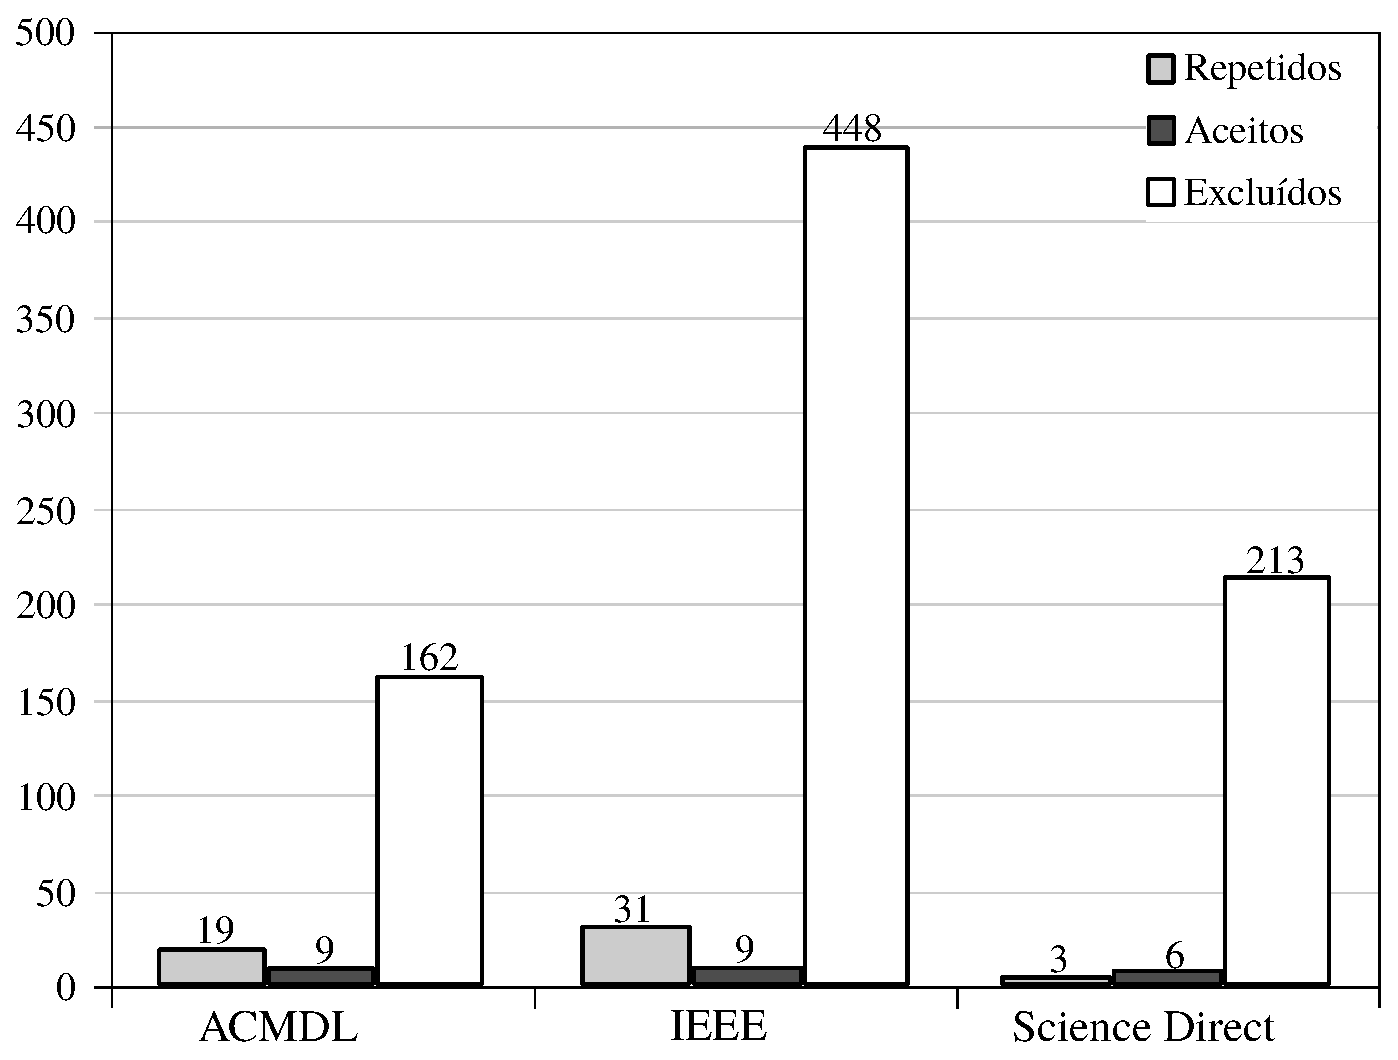
\includegraphics[width=7.5cm, height=5cm]{./secoes/correlatos/pics/img/GraficoQuantidade.eps}
  \caption{Agrupados por base de dados}
  \label{fig:figArtigosPorBase}
\end{subfigure}%
\begin{subfigure}{.5\textwidth}
  \centering
  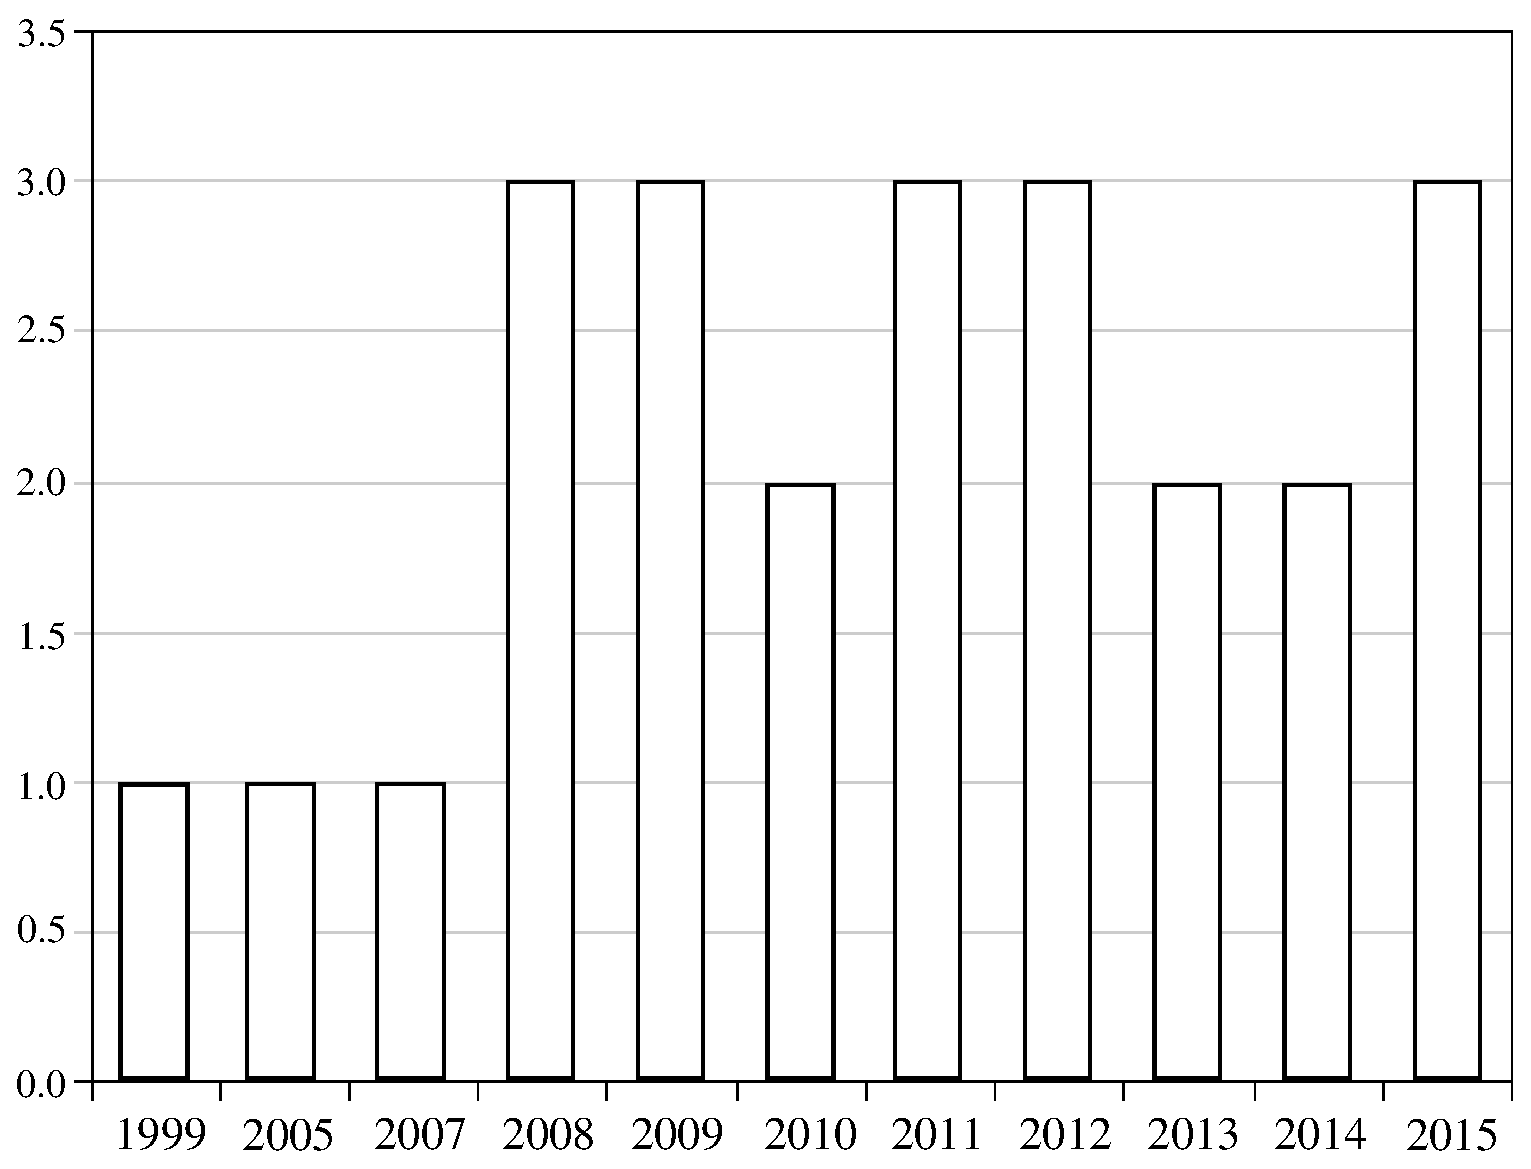
\includegraphics[width=7.5cm, height=5cm]{./secoes/correlatos/pics/img/GraficoQuantidadeAno.eps}
  \caption{Agrupados por ano de publicação}
  \label{fig:figArtigosPorAno}
\end{subfigure}
\label{fig}
\vspace{0.1cm}
 \source{\varAutorData}
\end{figure}

\subsection{Extração de dados}
Os dados extraídos de cada um dos artigos podem ser vistos na tabela \ref{tabResumoTecnicas}, junto com suas respectivas referências.

{\tiny
%	Abre ambiente para tabelas com mais de uma página.
\begin{longtabu} to \textwidth { |X[2.5,l]<{\strut}| X[2.0,l]<{\strut}| X[3.5,l]<{\strut}| }

%	Legenda e rótulo.
\caption{Técnicas da literatura correlata} \label{tabResumoTecnicas}
\\ \hline

%	Cabeçalho da primeira paǵina.
\multicolumn{1}{|c|}{\textbf{Referência}} & 
\multicolumn{1}{c|}{\textbf{Técnica}} & 
\multicolumn{1}{c|}{\textbf{Validação}} \\ \hline \endfirsthead

%	Cabeçalho repetido em todas as páginas.
\multicolumn{3}{c}
{ \tablename\ \thetable{} -- Continuação da página anterior} \\
\hline \multicolumn{1}{|c|}{\textbf{Referência}} &
\multicolumn{1}{c|}{\textbf{Técnica}} &
\multicolumn{1}{c|}{\textbf{Validação}}  \\ \hline
\endhead

%	Rodapé repetido em todas as páginas.
\hline \multicolumn{3}{|r|}{{Continua na próxima página}} \\ \hline
\endfoot
\endlastfoot
\cite{Telea1999}			& Frequência 							& Estudo de caso									\\ \hline

\cite{Bomfim2005}			& Ontologia 							& Estudo de caso									\\ \hline
	                 	
\cite{Shao2007}				& \emph{Itemsets} e proveniência de execução	& Estudo de caso									\\ \hline
                  	
\cite{Koop2008}				& Frequência e proveniências 			& \emph{Workflows} e suas proveniências				\\ \hline
                  	
\cite{Oliveira2008}			& Proveniências							& Estudo de caso									\\ \hline
                  	
\cite{Wang2008}				& Entrada e saída de atividades  		& Estudo de caso									\\ \hline
                  	
\cite{Shao2009}				& Proveniência de execução				& Estudo de caso									\\ \hline
                  	
\cite{Wang2009}				& \emph{Itemsets} e proveniência de execução	& Estudo de caso									\\ \hline
                  	
\cite{Zhang2009}			& Proveniência de modelagem				& Usados \emph{workflows} sintéticos 				\\ \hline 
                  	
\cite{Leng2010}				& Planejador							& Estudo de caso									\\ \hline 

\cite{Oliveir2010}			& Frequência							& Comparação com \citeonline{Koop2008}				\\ \hline 
                 	
\cite{Cerezo2011}	  		& Entrada/saída e semântica				& Estudo de caso									\\ \hline
                 	
\cite{Tan2011}				& Proveniência de execução				& Estudo de caso									\\ \hline 
                 	
\cite{Zhang2011}			& Frequência							& Dados do \emph{myExperiment} \cite{ROURE2015}		\\ \hline 
                 	
\cite{Cao2012}				& Proveniência de modelagem				& Comparado com \citeonline{Zhang2009}				\\ \hline 
                 	
\cite{Diamantini2012}		& Proveniência de modelagem				& Dados do \emph{myExperiment} \cite{ROURE2015}		\\ \hline 
                 	
\cite{Yao2012}				& Baseado em confiança					& Dados do \emph{myExperiment} \cite{ROURE2015}		\\ \hline
                 	
\cite{Garijo2013}			& Frequência e proveniência de execução	& Dados do SGWC \emph{Wings} \cite{Wings2015} 		\\ \hline 
                 	
\cite{Yeo2013}				& Proveniência de execução				& Dados do \emph{myExperiment} \cite{ROURE2015}		\\ \hline 
		
\cite{Zhang2014}			& Frequência e anotações			 	& Interfaces do \cite{ProgrammableWeb}				\\ \hline 

\cite{CorchoGarijo2014} 	& Frequência e Ontologia			  	& Dados da plataforma LONI \cite{Rex2003}			\\ \hline

\cite{TostaBraganholo2015}	& \emph{Itemsets} considerando ordem	& Comparação com \citeonline{Koop2008}				\\ \hline

\cite{Mohan2015}			&  Entrada/saída e semântica			& Dados do \emph{myExperiment} \cite{ROURE2015}		\\ \hline

\cite{Soomro2015}			& Frequência e Ontologia				& Dados da plataforma LONI \cite{Rex2003}			\\ \hline
\caption*{{\footnotesize Fonte: \varAutorData } }
\end{longtabu}
%\source{\varAutorData}
%\source{\varAutorData}
}

\section{Análise dos artigos selecionados pela revisão sistemática}\label{SEC_RESULTADOS_REVISAO}
Nesta seção são apresentadas as técnicas para recomendar atividades em \emph{workflows} científicos, empregadas ou propostas pelos trabalhos retornados pela revisão da seção \ref{SEC_METODOLOGIA_REVISAO}.

O sistema \emph{Smartlink}, proposto por \citeonline{Telea1999}, modela os \emph{workflows} científicos como grafos, nos quais as arestas correspondem ao fluxo de dados e os nós às atividades. É criado um grafo das atividades mais utilizadas e elaborada uma busca em profundidade procurando por atividades. A recomendação do \emph{Smartlink} é baseada no grafo de atividades mais utilizadas, o que permite minimizar os seguintes problemas: i) Como conectar duas atividades?; e ii) Quais atividades podem ser conectadas a uma atividade específica? A estratégia de recomendação não foi testada e comparada com a literatura, foi apenas implementada em alguns sistemas e usada.

\citeonline{Bomfim2005} desenvolveram um sistema de recomendação de atividades em \emph{workflows} científicos baseado em ontologia de domínio que é utilizada para recomendar atividades em \emph{workflows}. São comparadas as anotações da proveniência de modelagem com as do \emph{workflow} em construção e são recomendados os \emph{workflows} que contenham os mesmos conceitos ontológicos. A proposta não considera as dependências de dados e de controle para recomendar atividades. Além disso, a qualidade da recomendação não foi testada e os autores não detalharam a ontologia construída.

\citeonline{Shao2007} e \citeonline{Shao2009} propõem minerar a proveniência de execução para encontrar os experimentos que terminam em estado de sucesso. As execuções dos \emph{workflows} são modeladas como grafos acíclicos dirigidos. Cada execução parte do estado inicial até atingir um dos estados finais: i) teste; ii) não finalizado; iii) irrelevante, que não auxilia a atingir o estado de sucesso; e iv) sucesso. São considerados críticos todos os caminhos que partem do estado inicial e terminam no estado sucesso. Não foram realizados experimentos sobre recomendação, apenas sobre tempo de execução para minerar a proveniência. Os autores citam que essas técnicas poderiam ser utilizadas para recomendar os \emph{subworkflows} de sucesso para os \emph{workflows} em construção.

\citeonline{Koop2008} recomenda \emph{subworkflows} frequentes considerando a estrutura do \emph{workflow}. Para tal, são encontradas (utilizando a proveniência de execução) todas as sequências de atividades posteriores ao nó âncora (aquele que vem antes do item a ser recomendado). Essas atividades serão recomendadas ao usuário. Os testes utilizaram \(2.875\) \emph{workflows} e suas proveniências de execução, geradas por estudantes durante um curso de visualização de dados. O conjunto de dados foi dividido em: i) treinamento, responsável por gerar caminhos; e ii) testes, responsável por usar caminhos gerados e recomendar.

\citeonline{Oliveira2008} propõem recomendar trechos de \emph{workflows} baseado em filtro colaborativo sobre a proveniência de execução e de modelagem de outros \emph{workflows}. Sempre que uma atividade é adicionada, o sistema verifica quais as atividades seguintes foram utilizadas, considerando os dados de proveniência, e recomendando-as. Esta estratégia não foi comparada com a literatura, foi apenas implementada no SGWC Vistrails \cite{Vistrails} e foi apresentada uma recomendação de uma atividade.

Na área de recomendação de serviços, \citeonline{Wang2008} recomendam serviços baseados nos fatores dependência entre serviços, modelos existentes e ordem de execução dos serviços. Considere um modelo de \emph{workflow} no qual um serviço ``b'' invoca um serviço ``c'' e o serviço ``c'' invoca o serviço ``d''. Em um \emph{workflow} em construção, após a inclusão do nó ``b'', serão dadas as recomendações ``c'' e ``d'' ordenadas pela proximidade com ``b''. A técnica foi testada em dois problemas da área de bioinformática, porém não ocorreu uma comparação com a literatura correlata.

\citeonline{Zhang2009} propõem uma estratégia de recomendação baseada no subgrafo anterior ao nó âncora (aquele que vem antes do item a ser recomendado) que é definido por meio da proveniência de modelagem. São recomendados os nós posteriores aos subgrafos com maior ocorrência, isto é, é gerada uma lista com todas as possibilidades de próximos nós baseados em todos os nós anteriores ao nó âncora, de acordo com a proveniência de modelagem. Esta estratégia foi testada por meio de \emph{workflows} e proveniências criados pelos autores.

\citeonline{Wang2009} recomendam atividades por meio de \emph{itemsets} frequentes minerados a partir das mudanças ocorridas nos \emph{workflows}. Cada mudança é denominada \(\Delta\), uma série destas transforma um \emph{workflow} em outro e consiste na sequência: \(\Delta_{0}, \Delta_{1}, \ldots, \Delta_{N}\). É aplicado o algoritmo \emph{Apriori} em todas as sequências de operações \(\Delta\). Dessa forma, são obtidas as regras de associação que podem ser usadas como recomendação. A técnica é implementada em um SGWC, porém não ocorrem comparações com a literatura correlata.

\citeonline{Leng2010} propõem um planejador que procura por termos de uma ontologia. Primeiramente, os grafos acíclicos dirigidos, que representam os serviços web e suas relações, são modelados como uma quíntupla (P, \(P_{0}\), G, A, \(\Gamma\)) onde P é o conjunto de proposições, \(P_{0}\) é o estado inicial, G é o estado a ser atingido, A é o conjunto de ações que transformam uma proposição em outra e \(\Gamma\) é a função que transforma proposições. 

No grafo, os serviços serão as ações A, as entradas e saídas de todos os serviços serão as proposições P, a entrada passada pelo usuário será o estado inicial \(P_{0}\) e a saída esperada pelo usuário será o estado final a ser atingido G. O planejador começa adicionando os estados que satisfaçam as entradas das proposições existentes e que tenham uma similaridade semântica mínima, a qual é calculada por meio de graus de similaridade comparando as anotações semânticas feitas em todos os serviços com termos controlados por uma  ontologia. 

A similaridade entre dois conceitos, \(c_{1}\) e \(c_{2}\), da ontologia é calculada com as seguintes regras: i) \(c_{1}\) e \(c_{2}\) são equivalentes, então é denominada exata; ii) \(c_{2}\) é super conceito de \(c_{1}\); iii) \(c_{1}\) é super conceito de \(c_{2}\); iv) são inexatos. Ao término do algoritmo é encontrado um caminho entre o estado inicial e o final o qual é recomendado. O sistema foi parcialmente testado, pois ainda estava sendo implementado, porém não ocorreram comparações com a literatura correlata, apenas uma recomendação específica para um caso simples.

\citeonline{Oliveir2010} recomenda atividades de \emph{workflows} científicos utilizando mineração sequencial. Essa abordagem permite utilizar uma modificação do algoritmo \emph{Preorder Linked WAP} (PLWAP) desenvolvido por \citeonline{Ezeife2005} para recomendar atividades. São determinadas as sequências maximais (aquelas que não estão presentes em outras sequências de um mesmo \emph{workflow}). As sequências são a entrada para o PLWAP que define os caminhos padrões (que são usados como recomendação). Foi usada uma base de dados de \(3.340\) \emph{workflows}, essa estratégia de recomendação foi comparada com a proposta por \citeonline{Koop2008}.

\citeonline{Cerezo2011} elaboraram um sistema que permite construir \emph{workflows} em alto nível, utilizando ontologias de domínio. Essa modelagem é convertida para uma linguagem que pode ser executada por sistemas gerenciadores de \emph{workflow} científico. Durante a tradução, que é semiautomática, são recomendados para o usuário \emph{subworkflows} que possuem entradas e saídas compatíveis sintaticamente e cuja similaridade ontológica é alta em relação ao \emph{workflow} de alto nível modelado. Os autores não citam a estratégia de validação dos resultados, apenas elaboram uma recomendação específica para um caso simples.

\citeonline{Tan2011} constroem dois grafos: i) \emph{workflows} e seus serviços, representados por nós, e as arestas representam a relação de inclusão de um serviço dentro de um \emph{workflow}; e ii) entre operações, em que os nós representam operações dentro de serviços e as arestas operações entre serviços. Com esses grafos, é possível usar o algoritmo \emph{Apriori} para descobrir quais serviços são utilizados em conjunto por quais usuários, e assim gerar recomendações. Não são citadas comparações com a literatura correlata, apenas uma recomendação específica para um caso simples.

\citeonline{Zhang2011} constroem redes sociais de: i) \emph{workflows} e serviços; ii) serviços e serviços; e iii) pessoas e serviços. As redes permitem avaliar quais serviços são utilizados por quais \emph{workflows}, com qual frequência e quem são os autores. O sistema foi testado com \emph{workflows} do repositórios \emph{myExperiment} \cite{ROURE2015} com validação cruzada, são recomendados os serviços mais frequentemente utilizados em \emph{workflows} distintos.

No contexto de processos de negócio, \citeonline{Cao2012} aplicam recomendação baseada em grafos durante a construção dos \emph{workflows}. Os grafos prontos são minerados para definir padrões (sequências frequentes). Em seguida, é calculada a distância entre os padrões e o processo de negócio (\emph{workflow}) em construção. Os padrões com menor distância em relação ao processo de negócio em construção são recomendados ao usuário. A distância é calculada utilizando uma métrica elaborada pelos autores que considera a posição do nó no modelo pronto e no subgrafo em construção. A técnica foi comparada com a proposta de \citeonline{Zhang2009}.

\citeonline{Diamantini2012} recomendam fragmentos de \emph{workflows}, modelados como um grafo dirigido acíclico, encontrando as menores subestruturas mais representativas de cada grafo. Para tal, empregam um algoritmo de agrupamento da biblioteca SUBDUE que permite reduzir os nós do grafo utilizando a métrica \emph{Minimum Description Length} (MDL)
\begin{align}
MDL = \frac{DL(S)+DL(G|S)}{DL(G)} \label{EQU_MDL}
\end{align}
em que \(DL(S)\) é a \emph{Description Length} (DL), que é uma função para computar o número de \emph{bits} necessários para representar a matriz de adjacência do subgrafo \(S\), \(DL(G)\) é a \emph{Description Length} do grafo original \(G\) e \(DL(G|S)\) \emph{Description Length} de \(G\) comprimido por \(S\). São recomendados os padrões mais representativos ordenados pelo valor da equação \eqref{EQU_MDL}. Para teste foi utilizado um subconjunto de \(564\) \emph{workflows} do repositório \emph{myExperiment} \cite{ROURE2015} obtendo como saída uma hierarquia de agrupamentos similares que, segundo os autores, poderiam ser usados para a recomendação.

\citeonline{Yao2012} recomendam com base na confiabilidade de serviços e autores: a \emph{ReputationNet} que é um sistema de recomendação de atividades para \emph{workflows} que considera a reputação do autor (escolaridade, especialidade e número de citações) e a popularidade dos serviços (frequência relativa). Os serviços mais populares dos autores mais confiáveis são recomendados. Foram utilizados diversos \emph{workflows} do repositório \emph{myExperiment} \cite{ROURE2015} para validar os resultados.

\citeonline{Garijo2013} mineram a proveniência de execução para encontrar fragmentos frequentes de \emph{workflows} e recomendá-los. Os rastros de proveniência são representados como grafos dirigidos acíclicos. Dado um repositório de \emph{workflows} e sua proveniência de execução, o objetivo é encontrar: i) conjuntos de atividades frequentes; e ii) \emph{subworkflows} frequentes, utilizando o algoritmo de agrupamento do SUBDUE (baseado na equação MDL). Os testes foram feitos com \(22\) \emph{workflows} e suas proveniências. O resultado de estruturas frequentes encontradas foi comparado com os resultados de uma pesquisa manual. A diferença entre esta proposta e a de \citeonline{Diamantini2012} é que esta considera a proveniência de execução para recomendar, a outra apenas os \emph{workflows} prontos.

\citeonline{Yeo2013} adaptam a técnica de rastro de causalidade para \emph{workflows} científicos, originalmente esta técnica foi usada em \emph{workflows} de negócios. Para isto, os autores armazenam a informação de fluxo dos dados junto com o grafo de causalidade para \emph{workflows} científicos 
\begin{align}
G = <N, DP, L_{B}, L_{A}>
\end{align}
em que \(N\) é o número de atividades, \(DP\) é o conjunto de caminhos do fluxo de dados, \((A, b) \in L_{B}\) é o conjunto de atividades anteriores, tal que a execução de \(b\) é sempre realizada após alguma atividade do conjunto \(A\) e \((a, B) \in L_{A}\) é o conjunto de nós posteriores, tal que \(a\) é sempre executada antes de alguma das atividades do conjunto \(B\).

Utilizando o rastro é possível criar um vetor de distâncias entre o nó âncora (que será alvo da recomendação) e os possíveis próximos nós, oriundos de \(L_{A}\). Esse vetor booleano contém o valor \emph{um} representando a presença de uma atividade do rastro e \emph{zero} caso contrário. Os vetores são gerados para todos os rastros da base de dados e suas similaridades são calculadas por meio da similaridade do cosseno \cite{Deza2009}. Foram usados \(12\) \emph{workflows} do repositório \emph{myExperiment} \cite{ROURE2015} modificados para receber a recomendação. A modificação consistia na remoção de uma atividade enquanto se esperava que o sistema a recomendasse.

\citeonline{Zhang2014} constroem uma rede social de \emph{workflows} e serviços (os quais são os nós) e suas possíveis relações (que são as arestas) são do tipo de inclusão ou de autoria. Essa rede pode ser modelada como uma matriz \(Q\) em que \(q_{i, j} = 1\) indica a inclusão do serviço \emph{i} no \emph{workflow} \emph{j} ou como a matriz \(S = Q^{T}Q\) em que \(s_{i, j}\) representa o número de \emph{workflows} nos quais os serviços (\(i, j\)) são chamados. 

Quanto mais vezes dois serviços são utilizados em \emph{workflows}, maior o grau de ligação entre os mesmos. Todos os serviços são publicados com metadados. Dessa forma, os autores calculam o \emph{Term Frequency-Inverse Category Frequency} (TF-ICF) nos metadados que descrevem os serviços e suas categorias. Com base nos valores de TF-ICF cada serviço é classificado em \(k\) categorias. Durante a construção do \emph{workflow} são sugeridos serviços de acordo com a métrica \emph{Rank-Biased Overlap} (RBO), descrita no artigo. São recomendados os serviços que possuem maior RBO em relação ao \emph{workflow} em construção. São usados serviços da plataforma \citeonline{ProgrammableWeb} para validar os resultados.

\citeonline{CorchoGarijo2014} recomendam atividades baseados em algoritmos de mineração de grafos para encontrar os \emph{subworkflows} mais frequentes e recomendá-los. A similaridade entre eles e o \emph{workflow} em construção é dada pela métrica MDL (ver equação \ref{EQU_MDL}). Como parâmetros, o usuário deve estabelecer o tamanho mínimo e máximo dos \emph{subworkflow} a serem recomendados. O algoritmo modela o problema como um grafo dirigido, em seguida calcula os fragmentos mais frequentes. Por fim, usa uma ontologia que relaciona os \emph{subworkflows} com os \emph{workflows}. Para validar a proposta, o sistema foi usado por usuários que compararam os \emph{subworkflows} gerados e sugeridos com \emph{subworkflows} que eles procuraram manualmente.

\citeonline{TostaBraganholo2015} recomendam atividades baseados em algoritmos de mineração sequencial (como \citeonline{Agrawal1994}), adaptados para considerar a ordem das atividades. A técnica pesquisa os \emph{itemsets} com confiança e suporte mínimos estabelecidos e recomenda-os durante a construção do \emph{workflow} científico considerando a ordem das atividades. Essa técnica foi comparada com o trabalho de \citeonline{Koop2008} (em termos de consumo de memória e tempo gasto para gerar subgrafos) para sua validação.
 
\citeonline{Mohan2015} desenvolveram uma plataforma \emph{web}, com a funcionalidade de recomendar \emph{workflows} finalizados da base de dados, a qual permite construir \emph{workflows} e anotá-los semanticamente usando \emph{tags} criadas pelo usuário. Durante a construção do \emph{workflow} o sistema pesquisa por todos os \emph{workflows} da base que contenham entrada compatível com a saída do \emph{workflow} em construção e analisa quais contêm as mesmas anotações semânticas que as do perfil do usuário e os recomenda. A validação ocorreu usando \(9.886\) usuários, \(2.664\) \emph{workflows} e \(9.624\) \emph{tags} do repositório \emph{myExperiment} \cite{ROURE2015}.

\citeonline{Soomro2015} criaram um sistema de recomendação baseado em mapeamento de atividades em conceitos ontológicos funcionais acrescido de semântica de dados oriunda de uma ontologia de domínio. Durante a construção do \emph{workflow}, cada uma de suas atividades é mapeada em um conceito ontológico, em seguida a base de dados recomenda todos os \emph{subworkflows} que contenham aqueles conceitos ontológicos naquela sequência ordenados pela sua frequência. Os testes foram realizados com \(65\) \emph{workflows} da plataforma LONI \cite{Rex2003} usando a métrica MRR. Os autores não citam detalhes da ontologia usada.

\section{Tendências observadas com os resultados da revisão sistemática}
A partir da figura \ref{figTecnicasPorQuantidade} é possível notar a existência de uma tendência no uso de técnicas baseadas em proveniência de dados, frequência e dependência da informação. A partir de \(2014\) a literatura começou a considerar estratégias híbridas que usam proveniência e algum tipo de informação semântica. No ano de \(2015\) foram publicados dois artigos propondo estratégias híbridas para recomendar que usam frequência e algum tipo de informação semântica para recomendar \emph{subworkflows}.
\begin{figure}[H]
	\centering
 	  \caption{Número de artigos por técnica de recomendação}
		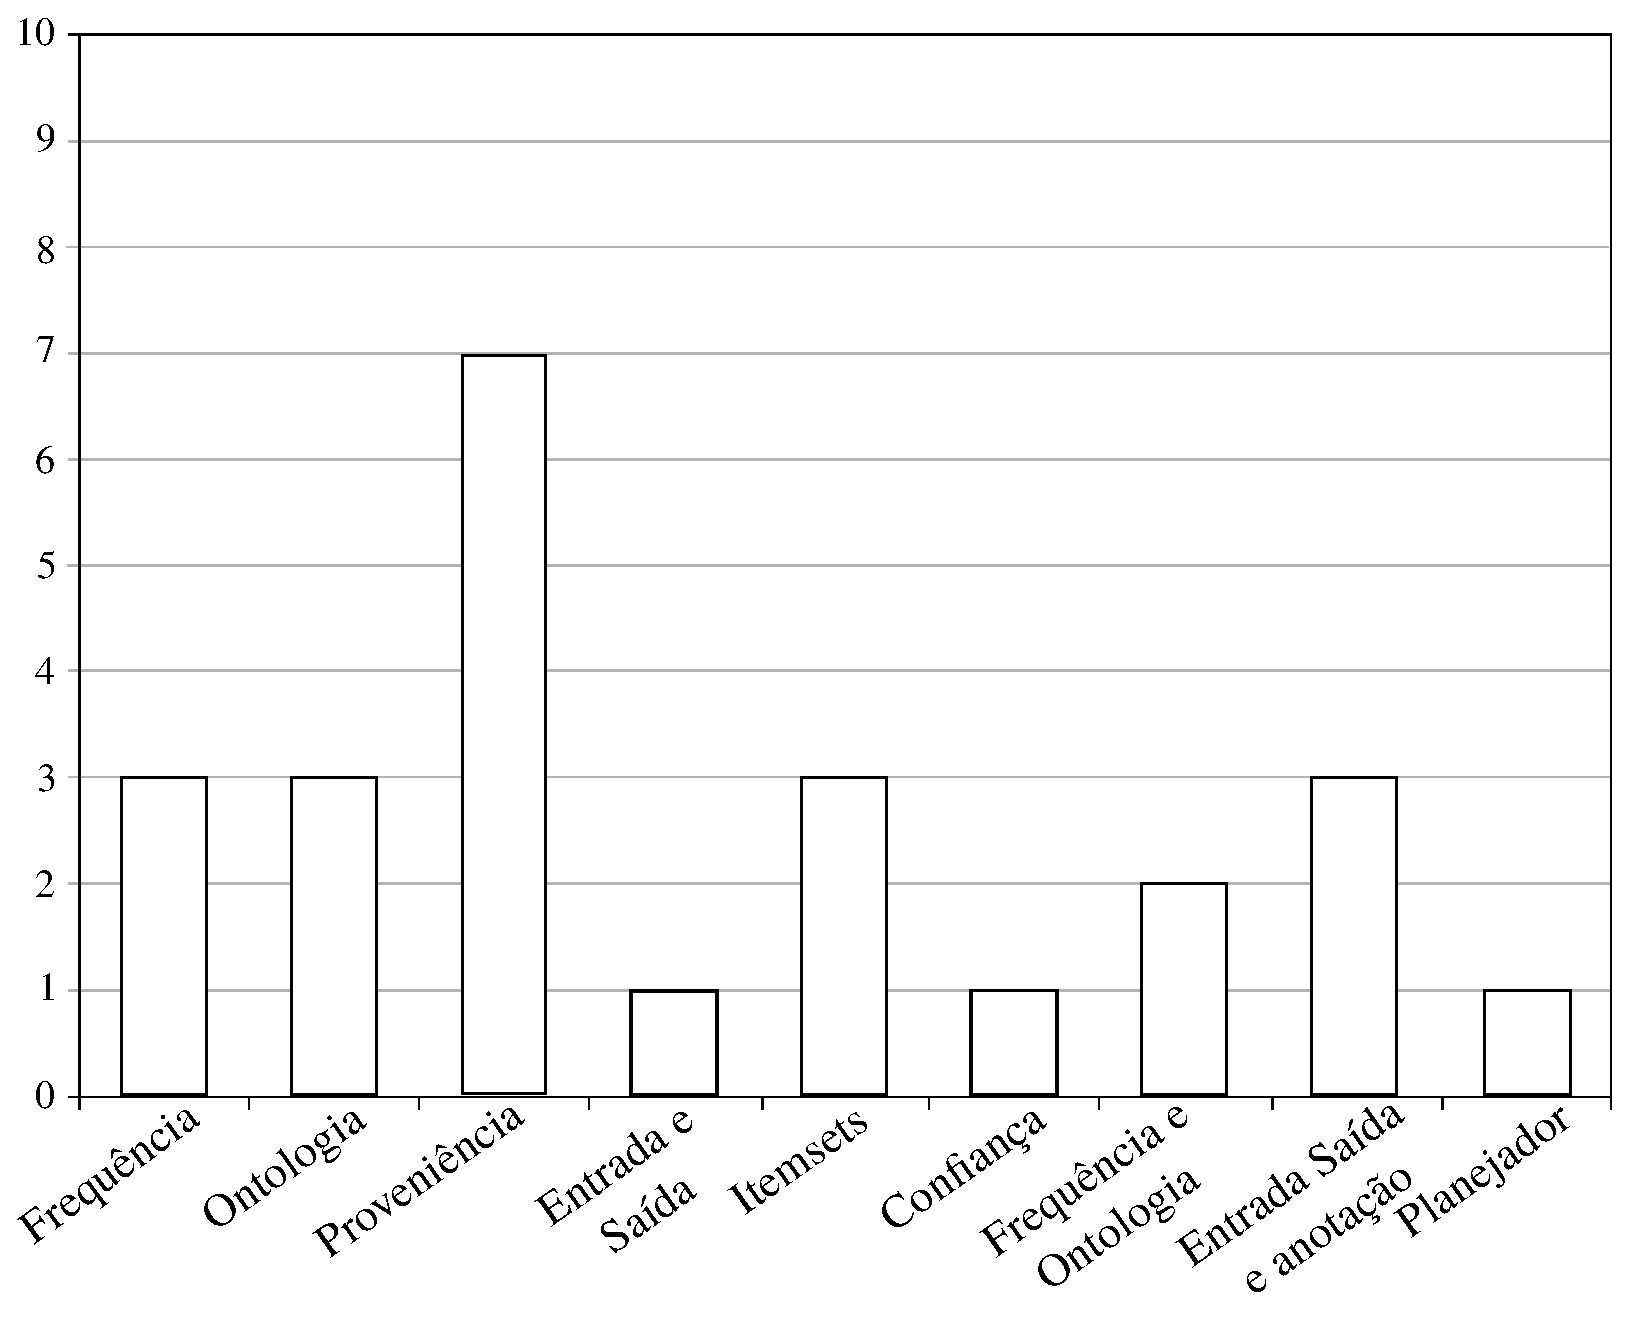
\includegraphics[width=11cm,height=6cm]{./secoes/correlatos/pics/img/GraficoQuantidadeTecnica.eps}
	\label{figTecnicasPorQuantidade}
  	\source{\varAutorData}
\end{figure}

A técnica baseada em proveniência de dados (mais utilizada na literatura) tem como vantagem considerar diversos dados históricos sobre um mesmo padrão de atividade. Por exemplo, para recomendar uma atividade em um \emph{workflow} que contenha a atividade~x, são considerados todos os \emph{workflows} que contenham x e suas atividades posteriores, a atividade com maior frequência é recomendada. Essa abordagem permite minimizar o efeito de \emph{outliers}. Como desvantagem, possui a necessidade de uma base de dados históricos relevantes, caso contrário, \emph{outliers} podem afetar o desempenho.

A técnica baseada em frequência tem como vantagem a simplicidade na implementação e como principal desvantagem a necessidade de uma base de dados com pouca esparsidade no uso de atividades.

A técnica baseada em dependência de informação tem como principal vantagem a facilidade de implementação. Como desvantagem, ela não leva em consideração a semântica dos dados das atividades. Por exemplo, uma \emph{string} que representa o nome de uma espécie de bactéria é considerada similar a uma \emph{string} que representa um CEP.

Outra tendência observada é sobre a validação dos resultados. Não há uma metodologia amplamente utilizada entre os trabalhos analisados para validação. Muitos autores apenas executam a solução uma vez para ``mostrar'' que sua solução funciona. Não ocorrem testes com dados sintéticos ou reais, o que pode ser verificado na tabela \ref{tabResumoTecnicas} em que \(11\) artigos estão nessa situação (marcados na tabela como ``Elaborado um estudo de caso'').

\section{Comparação da solução proposta com os trabalhos correlatos}\label{SEC_COMPARACAO_CORRELATOS}
Nesta seção são comparadas as técnicas descritas com o projeto deste mestrado em relação as restrições típicas de sistemas de recomendação de \emph{workflows} científicos, que foram detalhadas na seção \ref{SEC_RECOMENDACAO_WORKFLOW_CIENTIFICO} do capítulo de conceitos fundamentais.

Os trabalhos de \citeonline{Shao2007} e \citeonline{Shao2009}, que consideram a mineração sequencial de atividades como \emph{itemsets} desconsideram a ordem das atividades e a semântica das mesmas. A proposta de \citeonline{TostaBraganholo2015} desconsidera apenas a semântica das atividades. Esta proposta de mestrado considera a ordem de atividades que é um fator importante na recomendação conforme visto no capítulo de conceitos fundamentais.

Os trabalhos de \citeonline{Koop2008, Oliveira2008, Wang2009, Zhang2009, Tan2011, Cao2012, Diamantini2012, Garijo2013, Yeo2013} consideram a ordem das atividades, entrada e saída e proveniência dos dados. Suas limitações são a necessidade de dados de proveniência, pois nem todo SGWC armazena essas informações, além de desconsiderar informação semântica dos \emph{workflows} e atividades. Este projeto não necessita de informações de proveniência e considera a semântica da informação por meio de uma ontologia hierarquizada e validada por um especialista da área.

O trabalho de \citeonline{Bomfim2005} usa apenas um mapeamento entre atividades e ontologia desconsiderando a entrada e saída, o que potencialmente gera recomendações ineficientes. Neste projeto são consideradas às entradas e saídas de cada atividade individualmente, além do uso de uma ontologia de domínio.

\citeonline{Wang2008, Leng2010} desconsideram o uso de semântica das atividades e da frequência de suas ocorrências em pares. Nesse projeto de mestrado são considerados esses dois fatores.

O trabalho de \citeonline{Yao2012} exige dados que permitam calcular a confiança dos usuários e dos seus \emph{workflows}. Repositórios como \emph{myExperiment} \cite{ROURE2015} não exigem dos usuários o preenchimento de todos os seus dados, de forma que grande parte das informações relacionadas a este aspecto não são preenchidas pelos usuários. Além disso, os autores desconsideram a semântica das atividades e \emph{workflows}. Este projeto de mestrado considera a semântica de \emph{workflows} e não necessita da informação sobre a confiança dos usuários.

Os trabalhos de \citeonline{Telea1999, Oliveir2010} e \citeonline{Zhang2011} desconsideram o uso de semântica de dados para recomendar, o que é um limitante conforme discutido por \citeonline{CorchoGarijo2014, Soomro2015}. No presente mestrado, a frequência é considerada em conjunto com a ontologia de domínio.

Os trabalhos de \citeonline{Zhang2014, Mohan2015, Cerezo2011} desconsideram o uso de uma ontologia hierarquizada e validada por um especialista. Dessa forma, a qualidade das anotações semânticas é questionável. Nesse projeto foi construída uma ontologia usando uma metodologia e esta foi validada por um especialista.

Os trabalhos de \citeonline{CorchoGarijo2014, Soomro2015} consideram o uso de frequência e ontologia, como neste projeto, porém recomendam \emph{subworkflows} o que limita as recomendações de atividades. Apenas atividades usadas em fragmentos comuns de \emph{workflows} poderão ser recomendadas. Em outras palavras, se a atividade se encontra no ``meio'' de um \emph{subworkflow} esta nunca poderá ser recomendada individualmente. No presente mestrado, todas as atividades tem possibilidade de ser recomendadas, mesmo que no final da lista de recomendação. Além disso, apresenta uma recomendação mais abrangente, pois trata o caso de atividades simples, \emph{subworkflows} e \emph{Shims} (ver seção \ref{SEC_CONSTRUCAO_WORKFLOWS_CIENTIFICOS}).

Neste mestrado o problema de recomendação de atividades foi também modelado como um problema de classificação e regressão, usando para isso \(5\) classificadores; \(5\) regressores; um classificador SVM composto (que usa o resultado dos outros classificadores e regressores para recomendar) e um \emph{ensemble} de classificadores (\emph{Rotation Forest}).

%
\chapter{Solu\c{c}{\~a}o proposta}\label{CAP_SOLUCAOPROPOSTA}
\begin{flushright}
	\textit{``Poder é sempre perigoso. Atrai o pior e corrompe o melhor. Nunca pedi por poder. Poder só é dado para aqueles que estão dispostos a abrir mão de si por ele.''\\
			(Ragnar Lothbrok)}
\end{flushright}

Este capítulo descreve a solução proposta para o problema de recomendar atividades em workflows científicos, que utiliza uma ontologia de domínio e frequência de atividades para recomendar atividades para cientistas durante a construção de \emph{workflows} científicos. Também são descritas as soluções propostas para o uso de classificadores e regressores para resolver o problema de recomendação de atividades, bem como o uso de um classificador composto e um \emph{ensemble} de classificadores.

Primeiramente será detalhado como a ontologia foi construída, qual a metodologia foi usada e o processo de sua construção. Em seguida será detalhado o conjunto de dados, como foram obtidos, sua organização em um modelo relacional e como ocorreu a modelagem desses dados para solucionar o problema de recomendação. O próximo passo é explicar as alterações necessárias nos dados para serem usados por classificadores e regressores. Em seguida, será explicada a estratégia de validação dos experimentos. Por fim, na última seção do capítulo, será detalhada a solução proposta que utiliza a ontologia construída.
 \usepackage[utf8]{inputenc}		% Codificacao do documento (conversão automática dos acentos)
 \usepackage{lastpage}			% Usado pela Ficha catalográfica
 \usepackage{indentfirst}		% Indenta o primeiro parágrafo de cada seção.
 \usepackage{color}				% Controle das cores
 \usepackage{graphicx}			% Inclusão de gráficos
 
 \usepackage{microtype} 			% para melhorias de justificação
 \DisableLigatures{encoding = *, family = *} %Remove ligaduras, tornando o texto bonito
 
 \usepackage{pdfpages}     		%para incluir pdf
 \usepackage{algorithm}			%para ilustrações do tipo algoritmo
 \usepackage{mdwlist}			%para itens com espaço padrão da abnt
 \usepackage[noend]{algpseudocode}			%para ilustrações do tipo algoritmo
 \usepackage{lipsum}				% para geração de dummy text
 \usepackage{subcaption}
 \usepackage{amsmath}
 \usepackage{epstopdf}
 \usepackage{array}
 \usepackage{graphicx}
 \usepackage{multirow}
 \usepackage{amstext}
 \usepackage{longtable, tabu}
 \usepackage[dvipsnames]{xcolor}
 \usepackage{amsfonts}
 \usepackage{bm}
 
\section{Desenvolvimento da ontologia}\label{SEC_DESENVOLVIMENTO_DA_ONTOLOGIA} 
A ontologia foi desenvolvida usando a metodologia \emph{Skeletal} \cite{Uschold95}, que contém as seguintes fases:
\begin{enumerate}
	\item Identificar a finalidade;
	\item Construção da ontologia:
	\begin{enumerate}
		\item Captura da ontologia;
		\item Codificação da ontologia;
		\item Integração com ontologias existentes;
	\end{enumerate}
	\item Validação;
	\item Documentação.
\end{enumerate}

A primeira fase, denominada \emph{Identificar a finalidade}, define o objetivo para o qual será construída a ontologia e como ela será utilizada futuramente. Neste projeto, a ontologia foi construída para agregar conhecimento semântico durante a recomendação de atividades, para tal, todos os \emph{workflows} de bioinformática foram anotados com os conceitos desta ontologia. A segunda fase, chamada de \emph{Construção da ontologia}, tem como objetivo construir a ontologia (usando uma linguagem formal) em três subfases: i) \emph{Captura da ontologia}; ii) \emph{Codificação da ontologia}; e iii) \emph{Integração com ontologias existentes}. 

Na primeira subfase são identificados os conceit\usepackage[utf8]{inputenc}		% Codificacao do documento (conversão automática dos acentos)
\usepackage{lastpage}			% Usado pela Ficha catalográfica
\usepackage{indentfirst}		% Indenta o primeiro parágrafo de cada seção.
\usepackage{color}				% Controle das cores
\usepackage{graphicx}			% Inclusão de gráficos

\usepackage{microtype} 			% para melhorias de justificação
\DisableLigatures{encoding = *, family = *} %Remove ligaduras, tornando o texto bonito

\usepackage{pdfpages}     		%para incluir pdf
\usepackage{algorithm}			%para ilustrações do tipo algoritmo
\usepackage{mdwlist}			%para itens com espaço padrão da abnt
\usepackage[noend]{algpseudocode}			%para ilustrações do tipo algoritmo
\usepackage{lipsum}				% para geração de dummy text
\usepackage{subcaption}
\usepackage{amsmath}
\usepackage{epstopdf}
\usepackage{array}
\usepackage{graphicx}
\usepackage{multirow}
\usepackage{amstext}
\usepackage{longtable, tabu}
\usepackage[dvipsnames]{xcolor}
\usepackage{amsfonts}
\usepackage{bm}
os e suas relações no domínio de aplicação. Para realizar esta subfase foi necessário estudar a área de alinhamento de sequências genômicas com os seguintes materiais de estudo: i) um livro \cite{Setubal97}; e ii) quatro cursos online, disponibilizados pela universidade de São Diego, criados por \citeauthoronline{Pevzner2015a} (\citeyear{Pevzner2015b}, \citeyear{Pevzner2015a}, \citeyear{Pevzner2015c}, \citeyear{Pevzner2015d}). 

A codificação da ontologia, realizada na segunda\usepackage[utf8]{inputenc}		% Codificacao do documento (conversão automática dos acentos)
\usepackage{lastpage}			% Usado pela Ficha catalográfica
\usepackage{indentfirst}		% Indenta o primeiro parágrafo de cada seção.
\usepackage{color}				% Controle das cores
\usepackage{graphicx}			% Inclusão de gráficos

\usepackage{microtype} 			% para melhorias de justificação
\DisableLigatures{encoding = *, family = *} %Remove ligaduras, tornando o texto bonito

\usepackage{pdfpages}     		%para incluir pdf
\usepackage{algorithm}			%para ilustrações do tipo algoritmo
\usepackage{mdwlist}			%para itens com espaço padrão da abnt
\usepackage[noend]{algpseudocode}			%para ilustrações do tipo algoritmo
\usepackage{lipsum}				% para geração de dummy text
\usepackage{subcaption}
\usepackage{amsmath}
\usepackage{epstopdf}
\usepackage{array}
\usepackage{graphicx}
\usepackage{multirow}
\usepackage{amstext}
\usepackage{longtable, tabu}
\usepackage[dvipsnames]{xcolor}
\usepackage{amsfonts}
\usepackage{bm}
 subfase, usou a ferramenta \emph{Protégé} \cite{Protege2014} por ter código aberto, ser muito conhecida na área de ontologias e permitir a utilização da linguagem formal de ontologias OWL \cite{W3COWL2015}. A terceira etapa, denominada \emph{Integração com ontologias existentes}, não ocorreu neste projeto pois não foram encontradas ontologias usadas para recomendar atividades em \emph{workflows} científicos na área de bioinformática.
\begin{figure}[hbt]
	\centering
 	\caption{Ontologia construída utilizando a metodologia \emph{Skeletal}}
		\includegraphics[width=6cm, height=8cm]{./secoes/solucaoProposta/pics/img/Ontologia.eps}
	\label{FIGURA_ONTOLOGIA_CONSTRUIDA}
	\vspace{0.1cm}
	\source{\varAutorData}
\end{figure}

A ontologia construída pode ser visualizada na figura \ref{FIGURA_ONTOLOGIA_CONSTRUIDA}, na qual os círculos são os conceitos do domínio e as linhas de ligação, são as relações entre conceitos. A relação que foi utilizada é a ``\emph{é subtipo de}''. Ao término da fase de construção, foi realizada a fase de validação da ontologia, realizada por um especialista no domínio de bioinformática. Que é orientador deste projeto, tem formação específica em bioinformática e \emph{workflows} científicos. A documentação da ontologia, que é a última etapa, foi realizada nesta seção da dissertação, na qual foram detalhados os motivos de sua construção, sua motivação, seus usos e a forma de sua validação.

\section{Modelagem dos dados}\label{SEC_MODELAGEM} 
Os \emph{workflows} foram obtidos no repositório \emph{myExperiment} \cite{ROURE2015}, por meio do \emph{software wget} \cite{wget2015}. Após efetuar o \emph{download} dos \(2481\) \emph{workflows} em formato \emph{xml}, foi utilizado o analisador de código \emph{Beautiful Soup} \cite{BeautifulSoup2015}, para organizar o conjunto de dados em uma base de dados relacional\footnote{www.each.usp.br/digiampietri/baseworkflows/SQL.tar.gz} (ver figura \ref{figura_modelo_conceitual}).
\begin{figure}[!hbt]
    \centering  
    \caption{Modelo de dados dos \emph{workflows} científicos}
    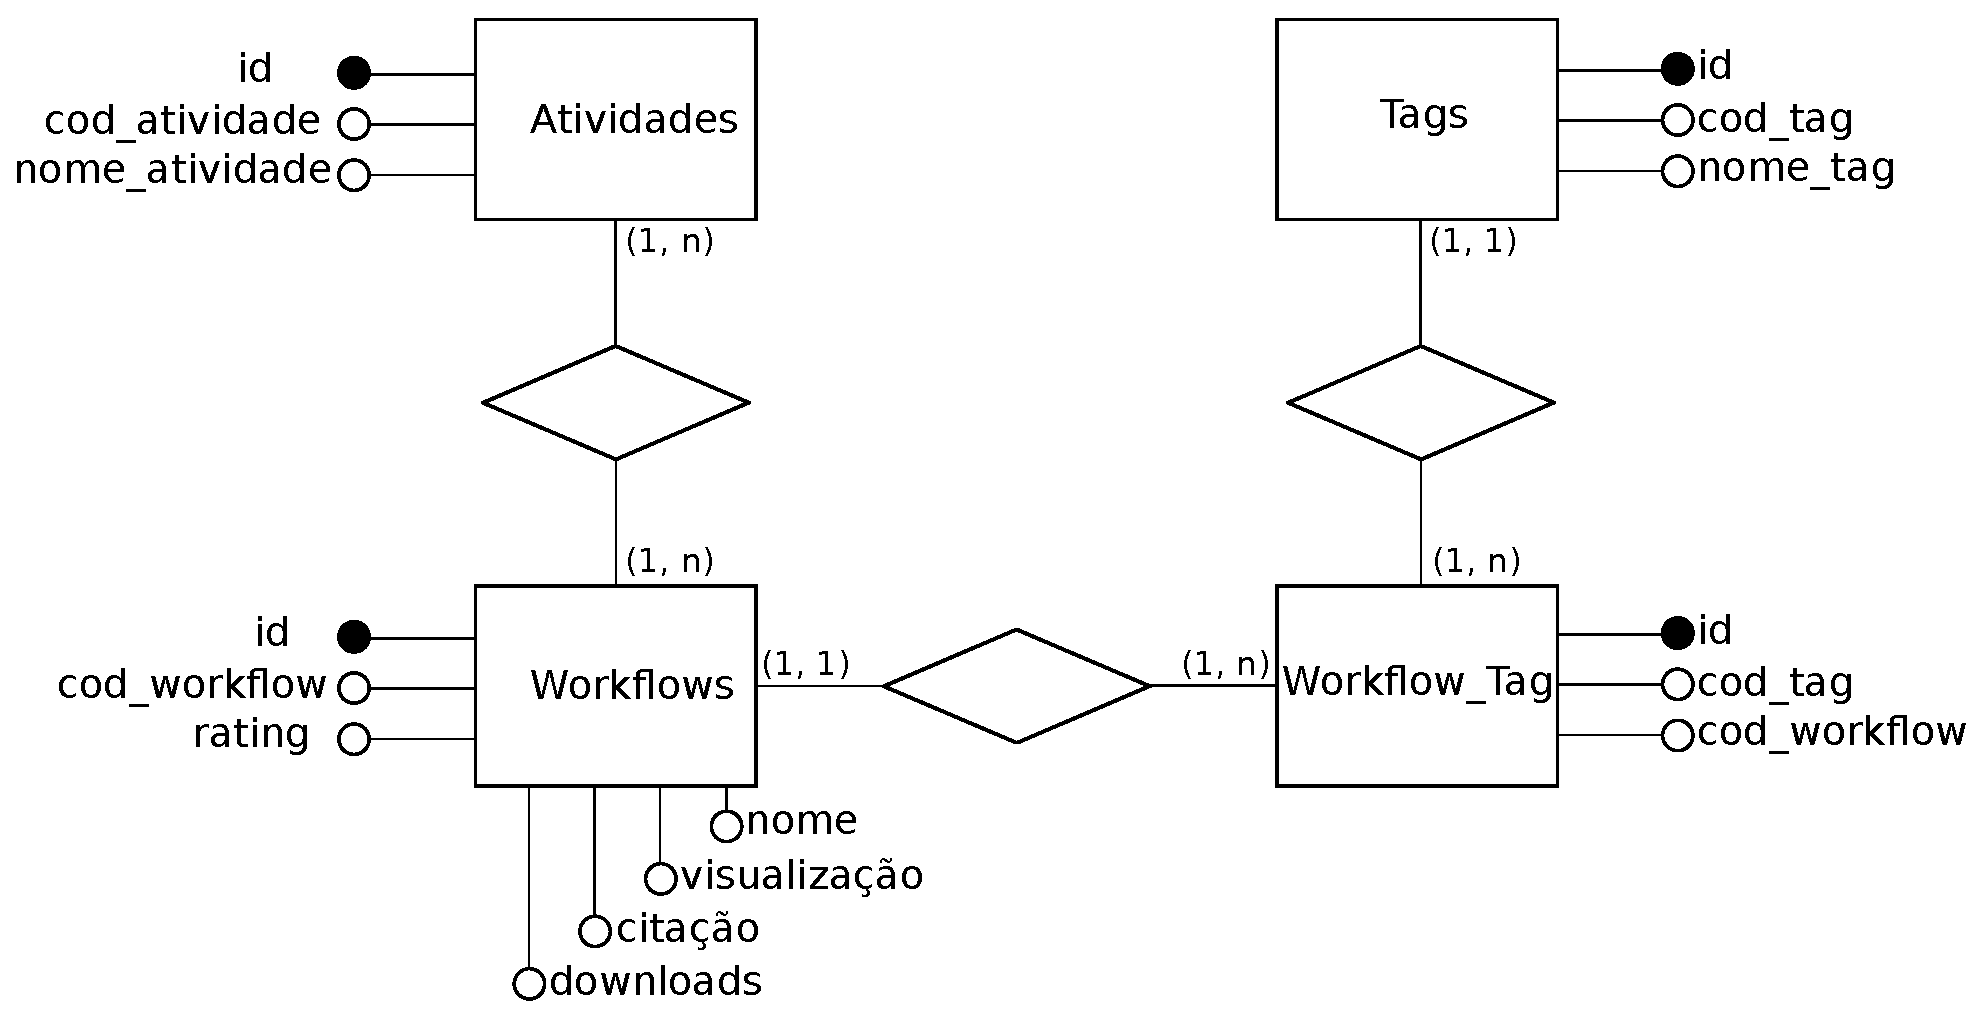
\includegraphics[width=10cm, height=4.5cm]{./secoes/solucaoProposta/pics/img/modelo_conceitual.eps}
    \label{figura_modelo_conceitual}
	\vspace{0.1cm}
    \source{\varAutorData}
\end{figure}
Neste modelo conceitual os retângulos representam as entidades, os losangos representam a relação entre atividades, os círculos brancos representam os atributos das entidades, os círculos pretos representam identificadores e os números próximos a cada entidade representam sua cardinalidade. Este modelo armazena todas as atividades dos \emph{workflows} (de diversas áreas) usando as entidades \emph{Atividades} e \emph{Workflow}. Para registrar qual a área científica (domínio de aplicação) de cada \emph{workflow} foram utilizadas as tabelas \emph{Workflow\_Tag} e \emph{Tag}.

Os \emph{workflows} da área de bioinformática (totalizando \(73\)) em conjunto com suas atividades (totalizando \(280\)) foram convertidos em uma matriz \(M_{i,j}\) em que cada linha \(i\) representa um \emph{workflow}, cada coluna \(j\) representa uma das \(280\) atividades e cada célula da matriz \(M\) representa a existência \(M_{i,j} = 1\), ou não \(M_{i,j} = 0\), da atividade da coluna \(j\) no \emph{workflow} \(i\). A tabela \ref{tabela_matriz_de_dados} apresenta um exemplo, fictício, de matriz \(M\). Para a realização dos testes, para cada linha da tabela \ref{tabela_matriz_de_dados} é removida uma atividade e é recomendada uma lista de possíveis atividades. O objetivo do sistema de recomendação é identificar corretamente qual a atividade está faltando no workflow (isto é, aquela que foi removida). 
\begin{table}[htb]
	\centering
	\caption{Exemplo de matriz de entrada.}
		\begin{tabular}{|c|c|c|c|c|}  \hline
		\textbf{\emph{Workflow}} & \textbf{Ativ \(\mathbf{01}\)} & \textbf{Ativ \(\mathbf{02}\)} & \textbf{\(\mathbf{\ldots}\)} & \textbf{Ativ \(\mathbf{280}\)}  \\ \hline
		01 			  & 1 			  & 0 			  & \(\ldots\) 	  & 0  				\\ \hline
		02 			  & 1 			  & 1 			  & \(\ldots\) 	  & 1  				\\ \hline
		03 			  & 1 			  & 0 			  & \(\ldots\) 	  & 1  				\\ \hline
		\(\vdots\) 		  			  & \(\vdots\) 	  & \(\vdots\) 	  & \(\vdots\) 	  & \(\vdots\) 		\\ \hline
		73 			  & 1 			  & 0 			  & \(\ldots\) 	  & 0  				\\ \hline
		\end{tabular}
	\label{tabela_matriz_de_dados}
	\vspace{0.1cm}
	\source{\varAutorData}
\end{table}

\section{Modelagem dos dados como problema de classificação e regressão}\label{SEC_MODELAGEM_CLASSIFICACAO_REGRESSAO} 
Para usar técnicas de classificação e regressão foram propostas algumas alterações no conjunto de dados original, descrito na tabela \ref{tabela_matriz_de_dados}, as quais podem ser visualizadas na tabela \ref{tabela_matriz_de_dados_adapatada_classificacao_regressao}. Cada \emph{workflow} foi replicado \(118\) vezes. Destes, \(59\) são uma cópia idêntica ao original, enquanto que dos outros \(59\) foi removida uma mesma atividade para todos os \emph{workflows}, e foi adicionada uma nova atividade representando uma possível recomendação. Dessa forma, para cada \emph{workflow} original haverá \(59\) instâncias corretas e \(59\) instâncias incorretas e este tipo de informação será utilizada para treinar os classificadores ou regressores.
\begin{table}[!htb]
	\tiny
	\centering
	\caption{Exemplo de matriz de entrada para técnicas de classificação e regressão}
	\begin{tabular}{|c|c|c|c|c|c|c|c|c|}  \hline
\textbf{\(\#\)} & \textbf{\emph{Workflow}} & \textbf{Ativ \(\mathbf{01}\)} & \textbf{Ativ \(\mathbf{02}\)} & \textbf{\(\mathbf{\ldots}\)}  & \textbf{Ativ \(\mathbf{279}\)} & \textbf{Ativ \(\mathbf{280}\)} & \textbf{Rótulo} \\ \hline

1	&		01		 			   & 1 			  & 0 			  & \(\ldots\) 	  & 0 & 0  			& T	\\ \hline
2	&		01 					   & 1 			  & 0 			  & \(\ldots\) 	  & 0 & 0  			& T	\\ \hline
\(\vdots\)  &  \(\vdots\) 	   	   & \(\vdots\)   & \(\vdots\) 	  & \(\vdots\) 	  & \(\vdots\) & \(\vdots\) & \(\vdots\)\\ \hline
59	&		01 					   & 1 			  & 0 			  & \(\ldots\) 	  & 0 & 0   		& T	\\ \hline
1	&		01		 			   & 0 (removida) 		  & 1 (adicionada) &\(\ldots\)& 1 & 0	& F	\\ \hline
2	&		01 					   & 0 (removida)& 0 		  & \(\ldots\) 	  & 1 (adicionada) & 0& F	\\ \hline
\(\vdots\)  &		\(\vdots\) 	   & \(\vdots\) & \(\vdots\) 	  & \(\vdots\) 	  & \(\vdots\) & \(\vdots\) & \(\vdots\) \\ \hline
59	&		01 					   & 0 (removida)			  & 0 			  & \(\ldots\) & 0 & 1 (adicionada)& F \\ \hline
					&\(\vdots\) & & & & & & 																		\\ \hline
1	&		73		 			   & 1 			  & 1  & \(\ldots\) 	  & 0 & 0  			& T	\\ \hline
2	&		73 					   & 1 			  & 1  & \(\ldots\) 	  & 0 & 0  			& T	\\ \hline
\(\vdots\)  &		\(\vdots\) 	   & \(\vdots\)   & \(\vdots\) 	  & \(\vdots\) 	  & \(\vdots\) & \(\vdots\) & \(\vdots\) \\ \hline
59	&		73 					   & 1 			  & 1  & \(\ldots\) 	  & 0 & 0   		& T	\\ \hline
1	&		73		 			   & 1 (adicionada) & 0 (removida)  & \(\ldots\) 	  & 1 & 0   		& F	\\ \hline
2	&		73 					   & 1 			  & 0 (removida)  & \(\ldots\)& 1 (adicionada) & 0  & F	\\ \hline
\(\vdots\)  &		\(\vdots\) 	   & \(\vdots\)   & \(\vdots\) 	  & \(\vdots\) 	  & \(\vdots\) & \(\vdots\) & \(\vdots\)	\\ \hline
59	&		73 					   & 1 			  & 0 (removida)  & \(\ldots\) 	  & 0 & 1 (adicionada) & F	\\ \hline
		\end{tabular}
	\label{tabela_matriz_de_dados_adapatada_classificacao_regressao}
	\vspace{0.1cm}
	\source{\varAutorData}
\end{table}

A escolha de \(59\) atividades a serem recomendadas foi feita por duas razões. A primeira é selecionar as 59 atividades com maior frequência na base de dados. A segunda é a limitação computacional: replicar as \(280\) possíveis recomendações poderia ser inviável em termos de treinamento. Foram replicadas \(59\) instâncias de \emph{workflows} idênticas consideradas corretas, isto é com a atividade correta não removida, para garantir o balanceamento entre classes. A última alteração foi adicionar uma coluna indicando se a recomendação da atividade proposta é a correta, isto é, a pertencente ao respectivo \emph{workflow} (\emph{T}) ou não (\emph{F}).

Na primeira modelagem, descrita na tabela \ref{tabela_matriz_de_dados}, cada linha (instância) recebe uma lista de atividades recomendadas pelas técnicas da literatura correlata e pela técnica proposta nesse mestrado (seção \ref{SEC_HIBRIDA_PROPOSTA}). Cada lista retornada segue algum critério de ordenação referente à técnica usada. Por exemplo, uma técnica baseada em frequência retorna uma lista de atividades ordenadas pelas suas frequências. 

Na segunda modelagem, cada linha classificada como \emph{não pertencente} (\emph{F}) ao \emph{workflow} é automaticamente adicionada no final da lista de recomendação. As outras atividades (\emph{T}) são adicionadas ao início da lista e ordenadas, de acordo com suas frequências, anotações ontológicas, ordem alfabética e seletor aleatório, nesta sequência de ordenações estáveis.

Esta modelagem foi utilizada pelos classificadores e regressores descritos no capítulo \ref{CAP_CONCEITOS_FUNDAMENTAIS}. Adicionalmente, os resultados desses classificadores e regressores foram utilizados pelo classificador composto e pelo \emph{ensemble} de classificadores. Essas estratégias que utilizam classificadores e regressores foram desenvolvidos de forma a não necessitarem de anotações semânticas dos \emph{workflows}.

Em ambas as modelagens, após construir a lista de recomendação oficial, aquela com os itens recomendados pelas técnicas, os sistemas de recomendação adicionam todas as outras atividades (que não foram recomendadas), ordenadas alfabeticamente, no final da lista. Dessa forma, todas as possíveis atividades estarão presentes na lista. Portanto as métricas descritas na seção \ref{SEC_METRICAS_VALIDACAO} sempre poderão ser calculadas.

\section{Estratégia de validação dos sistemas de recomendação} \label{SEC_METRICAS_VALIDACAO}
Para a validação será utilizada a técnica cruzada considerando \(10\) subconjuntos (\emph{\(10\)-fold cross validation}). Nessa técnica, o conjunto de dados é dividido em 10 subconjuntos (\emph{folds}) e são realizadas dez execuções. Em cada uma, \(10\%\) dos \emph{workflows} são separados para teste e \(90\%\) para treinamento. Assim, para cada execução, o sistema treina com \(90\%\) dos dados e o resultado do treinamento é testado para os \(10\%\) restantes. 

Deve-se ressaltar que \(100\%\) do conjunto de dados é rotulado (isto é, fica explícito ao sistema qual atividade foi removida) e assim é possível verificar o desempenho de cada uma das execuções. O teste apresenta os \(10\%\) de \emph{workflows}, sem informar os rótulos (a atividade removida), para os sistemas de recomendação que já foram treinados. Ao término das dez execuções são calculadas as médias das métricas: i) \emph{Sucess at rank k} (\(S@k\)); e ii) \emph{Mean Reciprocal Rank} (MRR). A figura~\ref{figura_10_fold_cross_validation} ilustra o processo de separação entre conjunto de treinamento e teste utilizado na estratégia de validação empregada.
\begin{figure}[!hbt]
	\centering   
	\caption{Exemplo de \emph{$10$-fold cross validation}}
	\includegraphics[width=14cm, height=9cm]{./secoes/conceitosFundamentais/pics/img/10FOLDCROSS.eps}
	\vspace{0.1cm}
	\source{Adaptado de \citeonline{HanKamber2011}}
	\label{figura_10_fold_cross_validation}
\end{figure}

A métrica \(S@k\) calcula a probabilidade de um item de interesse estar localizado entre as \(k\) primeiras posições da lista de atividades recomendadas. Seus valores residem entre zero e um. Os resultados dessa métrica são cumulativos para valores crescentes de \(k\), isto ocorre pois se uma atividade de interesse estiver entre as cinco primeiras posições da lista de recomendações, ela também encontra-se entre as dez primeiras posições. No limite, a atividade sempre estará entre as \(L\) primeiras posições, sendo \(L\) o tamanho total da lista de recomendações. Assim, valores elevados para $S@k$ são considerados bons, especialmente para valores baixos de $k$. O cálculo dessas métricas é detalhado pelas equações \cite{Harvey2010}:
\begin{align}
MRR &= \frac{1}{N} \sum\limits_{i=1}^{N} \left( \frac{1}{n_{i}} \right) 		\label{equ_mrr}\\
S@k &= \frac{1}{N} \sum\limits_{i=1}^{N} \left( I(n_{i} \leq k) \right)			\label{equ_s@k}
\end{align}
em que \(N\) é o número de listas recomendadas, \(n_{i}\) é a posição do item desejado na lista de recomendações \(i\), \(k\) é uma posição da lista determinada como parâmetro de entrada da equação \eqref{equ_s@k} e a função \emph{I}, indica se a atividade \(n_{i}\) ocorre em uma posição (\(x\)) menor ou igual ao parâmetro de entrada \(k\), e é dada por
\begin{align}
I(x, k)   &= \begin{cases} \label{equ_indicativa}
1 \textrm{ se } x \leq k \\
0 \textrm{ caso contrário }
\end{cases}
\end{align}

Para exemplificar o uso destas métricas será utilizado um \emph{workflow} fictício representado na figura \ref{figura_atividades_removidas} que teve quatro atividades removidas (\textbf{B}, \textbf{C}, \textbf{A} e \textbf{Z}) uma a uma gerando quatro casos que necessitam de recomendações (\(\mathbf{1}, \mathbf{2}, \mathbf{3}\) e \(\mathbf{4}\)). Que foram usados como entradas para quatro sistemas de recomendação distintos. Cada sistema produziu quatro listas de recomendação, uma para cada caso da figura \ref{figura_atividades_removidas}, rotulados com a mesma numeração. Assim, a lista \(01\) é a recomendação correspondente do caso \(1\) e assim sucessivamente.
\begin{figure}[!hbt]
	\centering   
	\caption{Quatro casos de recomendação de atividades}
	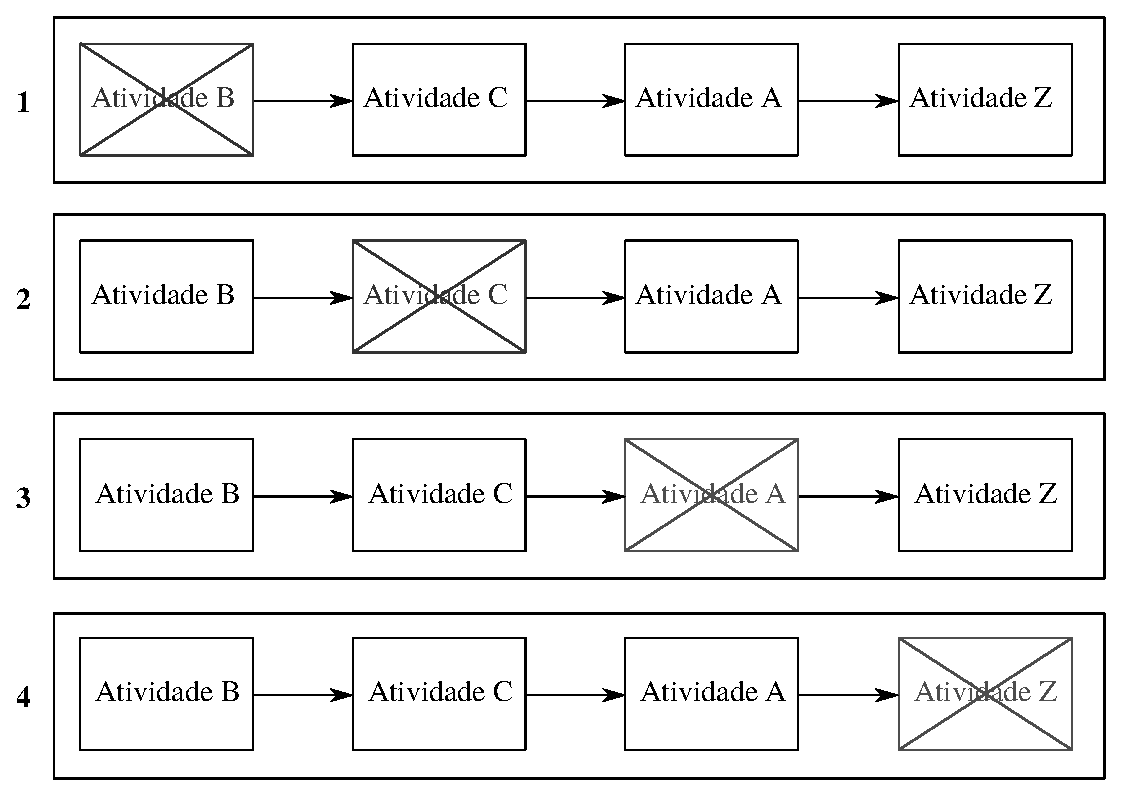
\includegraphics[width=13cm, height=7cm]{./secoes/conceitosFundamentais/pics/img/atividadeRemovida.eps}
	\vspace{0.1cm}
	\source{\varAutorData}
	\label{figura_atividades_removidas}
\end{figure}

As tabelas \ref{TABELAO:SISTEMA_RECOMENDACAO_01}, \ref{TABELAO:SISTEMA_RECOMENDACAO_02}, \ref{TABELAO:SISTEMA_RECOMENDACAO_03} e \ref{TABELAO:SISTEMA_RECOMENDACAO_04} apresentam os resultados dos quatro sistemas de recomendação. Cada item em negrito das listas representa a atividade que foi removida do \emph{workflow}, que é o item considerado correto (atividades com \emph{X} na figura \ref{figura_atividades_removidas}). Sua posição é determinada na coluna \emph{Rank} dessas tabelas.
\begin{table}[!htb]
	\tiny
	\caption{Exemplo de sistemas de recomendações de atividades}
	\begin{subtable}{.5\linewidth}
		\centering
		\begin{tabular}{|c|l|l|l|l|} \hline 
			\textbf{Rank} & \textbf{Lista} \(\mathbf{01}\) & \textbf{Lista} \(\mathbf{02}\) & \textbf{Lista} \(\mathbf{03}\) & \textbf{Lista} \(\mathbf{04}\) \\ \hline 
			1                & Ativ\_A	     		& Ativ\_H    			& Ativ\_Z   		& Ativ\_I    		\\
			2                & \textbf{Ativ\_B}		& Ativ\_B   			& Ativ\_E   		& Ativ\_C 			\\
			3                & Ativ\_C    			& Ativ\_I    			& \textbf{Ativ\_A}  & Ativ\_Z  			\\
			4                & Ativ\_D   			& Ativ\_X    			& Ativ\_X    		& Ativ\_B			\\
			5                & Ativ\_E   			& Ativ\_A			 	& Ativ\_C    		& Ativ\_S			\\
			6                & Ativ\_F   			& Ativ\_D    			& Ativ\_D    		& Ativ\_N			\\
			7                & Ativ\_G   			& \textbf{Ativ\_C}  	& Ativ\_Q    		& Ativ\_K			\\
			8                & Ativ\_H   			& Ativ\_Z    			& Ativ\_B   		& \textbf{Ativ\_Z}	\\
			9                & Ativ\_I    			& Ativ\_P   			& Ativ\_F   		& Ativ\_H			\\
			10               & Ativ\_Z   			& Ativ\_F    			& Ativ\_K    		& Ativ\_A			\\ \hline
		\end{tabular}
		\caption{Sistema de recomendação \(01\)}   
		\label{TABELAO:SISTEMA_RECOMENDACAO_01}		
	\end{subtable}%
	\begin{subtable}{.5\linewidth}
		\centering
		\begin{tabular}{|c|l|l|l|l|} \hline 
			\textbf{Rank} & \textbf{Lista} \(\mathbf{01}\) & \textbf{Lista} \(\mathbf{02}\) & \textbf{Lista} \(\mathbf{03}\) & \textbf{Lista} \(\mathbf{04}\) \\ \hline 
			1                & Ativ\_A	     		& \textbf{Ativ\_C}		& \textbf{Ativ\_A}	& Ativ\_I                    \\
			2                & \textbf{Ativ\_B} 	& Ativ\_B   			& Ativ\_E   		& Ativ\_C 	                 \\
			3                & Ativ\_C    			& Ativ\_I    			& Ativ\_Z			& Ativ\_A                    \\
			4                & Ativ\_D   			& Ativ\_X    			& Ativ\_X    		& \textbf{Ativ\_Z}           \\
			5                & Ativ\_E			   	& Ativ\_A			  	& Ativ\_C    		& Ativ\_S	                 \\
			6                & Ativ\_F   			& Ativ\_D    			& Ativ\_D    		& Ativ\_N                    \\
			7                & Ativ\_G   			& Ativ\_H    			& Ativ\_Q    		& Ativ\_K	                 \\
			8                & Ativ\_H   			& Ativ\_Z    			& Ativ\_B   		& Ativ\_U	                 \\
			9                & Ativ\_I    			& Ativ\_P   			& Ativ\_F   		& Ativ\_H	                 \\
			10               & Ativ\_Z   			& Ativ\_F    			& Ativ\_K    		& Ativ\_X	           \\ \hline
		\end{tabular}
		\caption{Sistema de recomendação \(02\)}
		\label{TABELAO:SISTEMA_RECOMENDACAO_02}
	\end{subtable}
	\\ \\ \hfill 
	\begin{subtable}{.5\linewidth}
		\centering
		\begin{tabular}{|c|l|l|l|l|} \hline 
			\textbf{Rank} & \textbf{Lista} \(\mathbf{01}\) & \textbf{Lista} \(\mathbf{02}\) & \textbf{Lista} \(\mathbf{03}\) & \textbf{Lista} \(\mathbf{04}\) \\ \hline 
			1                & Ativ\_A			    & Ativ\_H    			& Ativ\_F   		& Ativ\_I                    \\
			2                & Ativ\_G    			& Ativ\_B   			& Ativ\_E   		& Ativ\_C 	                 \\
			3                & Ativ\_C    			& Ativ\_I    			& Ativ\_Z			& Ativ\_A                    \\
			4                & Ativ\_D   			& Ativ\_X    			& Ativ\_X    		& Ativ\_B	                 \\
			5                & Ativ\_E   			& Ativ\_A	  			& Ativ\_C    		& Ativ\_S	                 \\
			6                & Ativ\_F   			& Ativ\_D    			& Ativ\_D    		& Ativ\_N                    \\
			7                & \textbf{Ativ\_B}		& Ativ\_Q				& Ativ\_Q    		& \textbf{Ativ\_Z}           \\
			8                & Ativ\_H   			& Ativ\_Z    			& Ativ\_B   		& Ativ\_U	                 \\
			9                & Ativ\_I    			& Ativ\_P   			& \textbf{Ativ\_A}	& Ativ\_H	                 \\
			10               & Ativ\_Z   			& \textbf{Ativ\_C}		& Ativ\_K    		& Ativ\_X           \\ \hline
		\end{tabular}
		\caption{Sistema de recomendação \(03\)}
		\label{TABELAO:SISTEMA_RECOMENDACAO_03}
	\end{subtable}%
	\begin{subtable}{.5\linewidth}
		\centering
		\begin{tabular}{|c|l|l|l|l|} \hline 
			\textbf{Rank} & \textbf{Lista} \(\mathbf{01}\) & \textbf{Lista} \(\mathbf{02}\) & \textbf{Lista} \(\mathbf{03}\) & \textbf{Lista} \(\mathbf{04}\) \\ \hline 
			1                & Ativ\_A			    & Ativ\_H    			& Ativ\_Z   		& \textbf{Ativ\_Z}           \\
			2                & Ativ\_Z    			& \textbf{Ativ\_C}		& Ativ\_E   		& Ativ\_C 	                 \\
			3                & Ativ\_C    			& Ativ\_I    			& Ativ\_Z			& Ativ\_A                    \\
			4                & Ativ\_D   			& Ativ\_X    			& Ativ\_X    		& Ativ\_B	                 \\
			5                & Ativ\_E   			& Ativ\_A			  	& Ativ\_C    		& Ativ\_X 	         		 \\
			6                & Ativ\_F   			& Ativ\_D    			& Ativ\_D    		& Ativ\_N                    \\
			7                & Ativ\_G   			& Ativ\_C    			& Ativ\_Q    		& Ativ\_K	                 \\
			8                & Ativ\_H   			& Ativ\_Z    			& Ativ\_B   		& Ativ\_U	                 \\
			9                & Ativ\_I    			& Ativ\_P   			& \textbf{Ativ\_A}	& Ativ\_H	                 \\
			10               & \textbf{Ativ\_B}  	& Ativ\_F    			& Ativ\_K    		& Ativ\_S		     \\ \hline
		\end{tabular}
		\caption{Sistema de recomendação \(04\)}
		\label{TABELAO:SISTEMA_RECOMENDACAO_04}
	\end{subtable}
	\label{TABELAO}
	\vspace{0.1cm}
	\source{\varAutorData}
\end{table}
O sistema de recomendação \(01\), cujos resultados se encontram na tabela \ref{TABELAO:SISTEMA_RECOMENDACAO_01}, apresenta os seguintes valores de \(S@k\)
\begin{align}
S@1 &= \frac{1}{4}  \Big( (I_{L_{1}} = 0) + (I_{L_{2}} = 0) + (I_{L_{3}} = 0) + (I_{L_{4}} = 0) \Big)	=	0,00	\\
S@3 &= \frac{1}{4}  \Big( (I_{L_{1}} = 1) + (I_{L_{2}} = 0) + (I_{L_{3}} = 1) + (I_{L_{4}} = 0) \Big)	=	0,50	\\
S@5 &= \frac{1}{4}  \Big( (I_{L_{1}} = 1) + (I_{L_{2}} = 0) + (I_{L_{3}} = 1) + (I_{L_{4}} = 0) \Big)	=	0,50	\\
S@7 &= \frac{1}{4}  \Big( (I_{L_{1}} = 1) + (I_{L_{2}} = 1) + (I_{L_{3}} = 1) + (I_{L_{4}} = 0) \Big)	=	0,75	\\
S@10 &= \frac{1}{4} \Big( (I_{L_{1}} = 1) + (I_{L_{2}} = 1) + (I_{L_{3}} = 1) + (I_{L_{4}} = 1) \Big) 	=	1,00		
\end{align}
sendo \(I_{L_{1}}\) o resultado da função indicadora \eqref{equ_indicativa}. As posições das atividades recomendadas por sistema são
\begin{align}
\left( \frac{1}{n_{i}} \right)_{L_{1}}  &= \frac{1}{2} 	\\
\left( \frac{1}{n_{i}} \right)_{L_{2}} &= \frac{1}{7} 	\\
\left( \frac{1}{n_{i}} \right)_{L_{3}} &= \frac{1}{3} 	\\
\left( \frac{1}{n_{i}} \right)_{L_{4}} &= \frac{1}{8} 	
\end{align}
e cuja média é dada por
\begin{align}
MRR &= \frac{\left( \frac{1}{2} + \frac{1}{7} + \frac{1}{3} + \frac{1}{8} \right)}{4} = 0,275297
\end{align}
De forma análoga os resultados obtidos pelos sistemas \(02\), \(03\) e \(04\) podem ser visualizados na tabela \ref{tabela_resultados_mrr_Sak}.
\begin{table}[!htb]
	\centering
	\caption{Lista de recomendação ordenada por frequência}
	\begin{tabular}{ccccccc} \hline
		\textbf{Sistema} & \(\mathbf{S@1}\) & \(\mathbf{S@3}\) & \(\mathbf{S@5}\) & \(\mathbf{S@7}\) & \(\mathbf{S@10}\) & \textbf{MRR}	\\ \hline
		1 & \(0,00\) 	& \(0,50\)	& \(0,50\)	& \(0,75\)	& \(1,00\) & \(0,275297\) \\ 
		2 & \(0,50\)	& \(0,75\)	& \(1,00\)	& \(1,00\)	& \(1,00\) & \(0,687500\) \\ 
		3 & \(0,00\)	& \(0,00\)	& \(0,00\)	& \(0,50\)	& \(1,00\) & \(0,124206\) \\ 
		4 & \(0,25\)	& \(0,50\)	& \(0,50\) 	& \(0,50\)	& \(1,00\) & \(0,427777\) \\ \hline
	\end{tabular}
	\label{tabela_resultados_mrr_Sak}
	\vspace{0.1cm}
	\source{\varAutorData}
\end{table}

Ao comparar os quatro sistemas é possível constatar que, de acordo com as métricas calculadas, o melhor é o número~\(02\) pois apresenta o maior valor de \(MRR = 0,687500\) e os maiores valores observados de \(S@1 = 0,50\) e \(S@3 = 0,75\).


\section{Solução híbrida de frequência e ontologia de domínio}\label{SEC_HIBRIDA_PROPOSTA} 
Uma outra solução proposta neste mestrado recomenda atividades usando três conceitos importantes na área de \emph{workflows} científicos: i) frequência de atividades; ii) compatibilidade entre entrada e saída; e ii) semântica de atividades. Para explicar esta proposta, será usada a figura \ref{FIGURA_ONTOLOGIA_CONSTRUIDA2} como exemplo. Nela é possível observar seis \emph{workflows} com suas anotações, que simulam uma base de dados de \emph{workflows} científicos.
\begin{figure}[!hbt]
	\centering
 	\caption{Exemplo de banco de dados de \emph{workflows} científicos}
		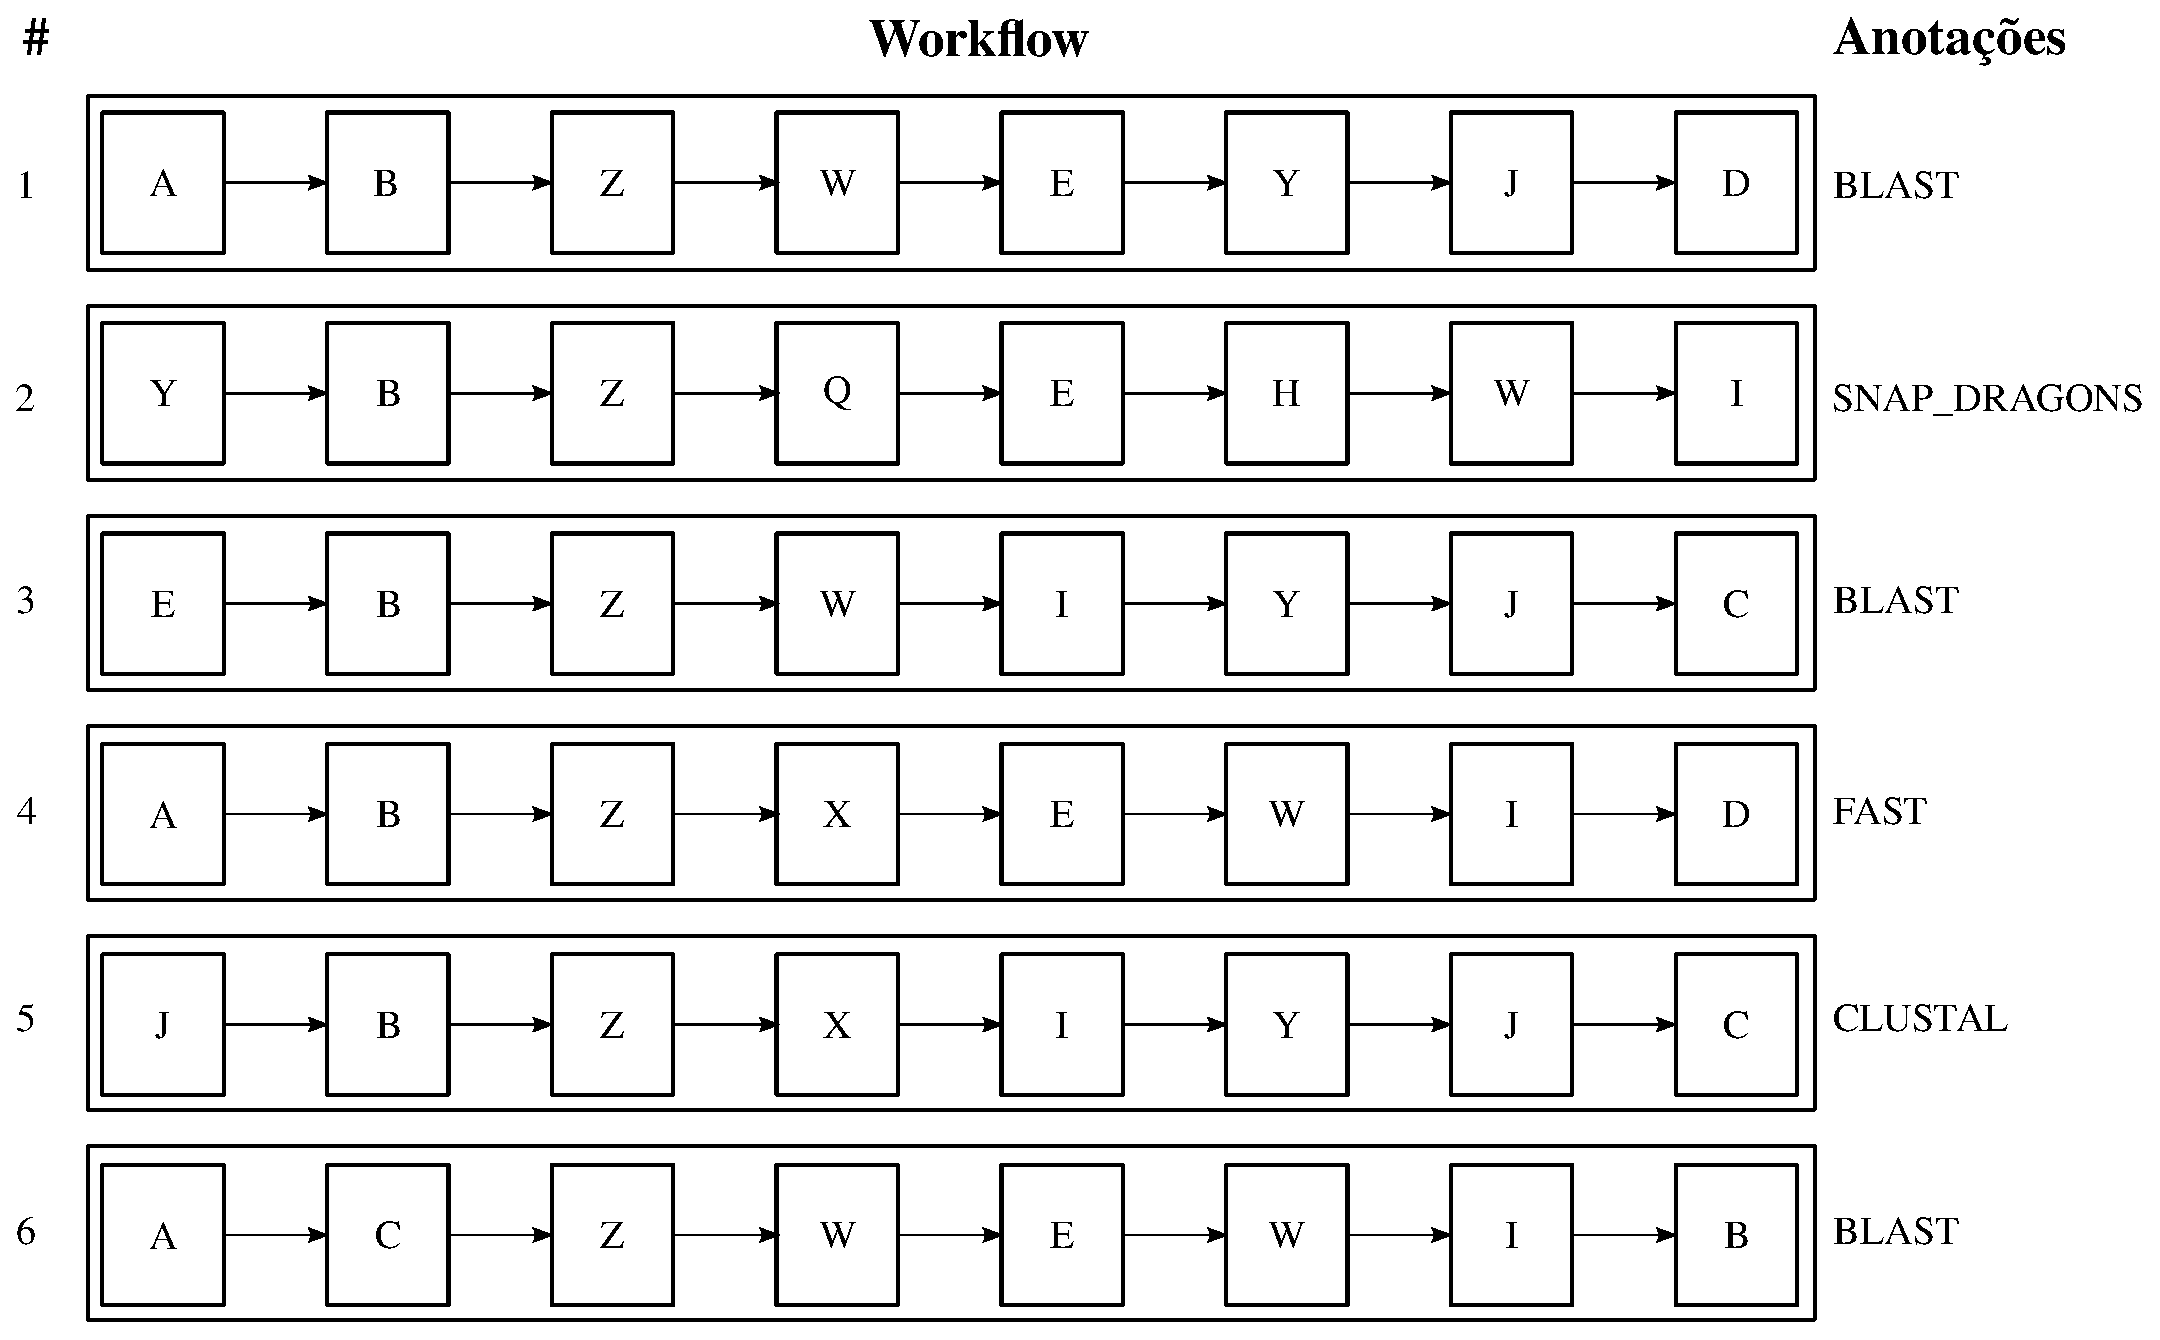
\includegraphics[width=12cm, height=7cm]{./secoes/solucaoProposta/pics/img/recomendacaofreqontologia.eps}
	\label{FIGURA_ONTOLOGIA_CONSTRUIDA2}
	\source{\varAutorData}
\end{figure}

A solução proposta começa calculando a frequência de ocorrência de cada par de atividades existentes, que é o número de vezes que uma atividade \emph{W} ocorre imediatamente após uma outra atividade \emph{Z}. Ao considerar somente atividades que já foram conectadas, previamente na base de \emph{workflows}, a compatibilidade de entrada e saída é garantida por consequência.

Após calcular a frequência é necessário anotar todos os \emph{workflows} da figura \ref{FIGURA_ONTOLOGIA_CONSTRUIDA2}, usando os conceitos da ontologia construída (ver figura \ref{FIGURA_ONTOLOGIA_CONSTRUIDA}). Essa etapa é feita manualmente (de forma não automatizada). Por fim, o algoritmo anota todas as atividades com as mesmas anotações de seus respectivos \emph{workflows}; isto é, se a atividade \emph{X} (da figura \ref{FIGURA_ONTOLOGIA_CONSTRUIDA2}) está dentro de dois \emph{workflows} com anotações distintas então esta atividade receberá duas anotações. O resultado final é a tabela \ref{tabela_lista_recomendacao_ordenada_frequencia}, que apresenta as frequências e anotações de atividades, nesse ponto o sistema está treinado e pronto para uso do cientista

Para compreender o mecanismo de recomendação treinado será usado outro exemplo, cujo objetivo é simular a interação do usuário com o sistema de recomendação. Suponha que durante a construção do \emph{workflow} \(1\) (ver figura \ref{FIGURA_ONTOLOGIA_CONSTRUIDA}) um cientista insira a atividade \emph{Z} e solicite uma recomendação. O sistema vai procurar na lista das atividades posteriores a \emph{Z} ordenadas por frequência e conceito ontológico e irá retornar a lista de recomendação apresentada na tabela~\ref{tabela_lista_recomendacao_ordenada_frequencia}. A ordenação por conceito ontológico, além de ser estável serve como critério de desempate, quando duas atividades tiverem a mesma frequência. Neste exemplo, de acordo com a lista de recomendação da tabela~\ref{tabela_lista_recomendacao_ordenada_frequencia}, a atividade \emph{W} seria recomendada em primeiro lugar ao cientista, o que representa um acerto.
\begin{table}[!htb]
	\centering
	\caption{Recomendação para a atividade \emph{Z} ordenada por frequência e conceito ontológico}
		\begin{tabular}{|c|c|c|c|}  \hline
		\textbf{Posição na Lista} & \textbf{Ativ} & \textbf{Frequência} & \textbf{Anotação Atividade} 	\\ \hline
		1				& W 				& 3 				& BLAST				\\ \hline
		2				& X 				& 2 				& FAST, CLUSTAL		\\ \hline
		3				& Q 				& 1 				& SNAP DRAGONS		\\ \hline
		\(\vdots\)		& \(\vdots\)		& \(\vdots\) 		& \(\vdots\)		\\ \hline
		280				& \(\vdots\)		& \(\vdots\)		& \(\vdots\)	\\ \hline
		\end{tabular}
	\label{tabela_lista_recomendacao_ordenada_frequencia}
	\vspace{0.1cm}
	\source{\varAutorData}
\end{table}

As atividades são anotadas com a mesma anotação dos \emph{workflows} que as contém. Dessa forma, é possível que haja pelo menos uma atividade com mais de uma anotação. Isso gera um novo caso de recomendação a ser considerado. Suponha que ambas as atividades \emph{W} e \emph{X} contenham dentro de suas listas de anotação o conceito \emph{BLAST}. Nesse caso, seria recomendada a atividade com menor número de anotações, por ser considerada mais específica para o experimento em questão. Caso ambas as atividades tenham o mesmo número de anotações, é utilizada a ordem alfabética de conceitos como critério de desempate. Se ocorrer um novo empate é usado um seletor aleatório.
%
\section{Comparação dos experimentos}

\begin{frame}		
	\begin{block}{Comparação dos experimentos}
		Resultados dos sistemas de recomendação.
		\bgroup
		\begin{table}[!htp]
			\centering
			\tiny
			\begin{tabular}{|l|l|l|l|l|l|l|l|l|} \hline
				\textbf{\(\mathbf{\#}\)} & \textbf{Técnica}&\textbf{S@1}&\textbf{S@5} & \textbf{S@10} & \textbf{S@50} & \textbf{S@100} & \textbf{S@280} & \textbf{MRR} \\ \hline
				
\rowcolor{roxo}		1  & Aleatório				& 0,0037 & 0,0260 & 0,0280 & 0,0300 & 0,0400 & 1,0000 & 0.033 \\ \hline
\rowcolor{roxo}		2  & \emph{Apriori}			& 0,0037 & 0,0385 & 0,0559 & 0,0568 & 0,0570 & 1,0000 & 0,037 \\ \hline
\rowcolor{amarelo}	3  & KNN\(_C\)				& 0,0037 & 0,0685 & 0,0959 & 0,5068 & 1,0000 & 1,0000 & 0,040 \\ \hline
\rowcolor{amarelo}	4  & Rede neural\(_C\)		& 0,0137 & 0,1507 & 0,1781 & 0,8082 & 1,0000 & 1,0000 & 0,089 \\ \hline
\rowcolor{amarelo}	5  & CART\(_C\)				& 0,0274 & 0,1233 & 0,3699 & 0,7671 & 1,0000 & 1,0000 & 0,113 \\ \hline
\rowcolor{amarelo}	6  & Naive Bayes\(_C\)     	& 0,0274 & 0,1507 & 0,3425 & 0,6301 & 1,0000 & 1,0000 & 0,114 \\ \hline
\rowcolor{verde}	7  & Binomial\(_R\) 		& 0,0822 & 0,1918 & 0,2055 & 0,8493 & 1,0000 & 1,0000 & 0,136 \\ \hline
\rowcolor{verde}	8  & Rede neural\(_R\)     	& 0,1096 & 0,2603 & 0,2603 & 0,2603 & 1,0000 & 1,0000 & 0,154 \\ \hline
\rowcolor{verde}	9  & MARS\(_R\)     		& 0,1233 & 0,2055 & 0,2192 & 0,7260 & 1,0000 & 1,0000 & 0,167 \\ \hline
\rowcolor{verde}	10 & SVM\(_R\)     			& 0,1233 & 0,3151 & 0,4932 & 0,8493 & 1,0000 & 1,0000 & 0,238 \\ \hline
\rowcolor{verde}	11 & CART\(_R\)    			& 0,1370 & 0,1370 & 0,2603 & 0,6164 & 1,0000 & 1,0000 & 0,114 \\ \hline
\rowcolor{roxo}		12 & FES           			& 0,1474 & 0,2603 & 0,3699 & 0,8671 & 1,0000 & 1,0000 & 0,196 \\ \hline
\rowcolor{amarelo}	13 & SVM\(_C\)    			& 0,2425 & 0,4658 & 0,4932 & 0,7123 & 1,0000 & 1,0000 & 0,244 \\ \hline
\rowcolor{azul}		14 & SVM composto\(_C\)		& 0,2515 & 0,4458 & 0,5232 & 0,7623 & 1,0000 & 1,0000 & 0,314 \\ \hline
\rowcolor{azul}		15 & Rotation Forest\(_C\)  & 0,2925 & 0,4558 & 0,5432 & 0,7723 & 1,0000 & 1,0000 & 0,324 \\ \hline
\rowcolor{vermelho}	16 & FESO          			& 0,3425 & 0,4658 & 0,5932 & 0,8123 & 1,0000 & 1,0000 & 0,334 \\ \hline
			\end{tabular}
			%\caption{Resultados dos sistemas de recomendação}
			%\label{tb_resultadosExperimentos}
			%\vspace{0.1cm}
			%\source{\varAutorData}
		\end{table}
		\egroup
		
	\end{block}
\end{frame}

%Falar isso, não devo ler
%\begin{frame}		
%	\begin{block}{Comparação}
%		A técnica FESO, proposta nessa dissertação, apresentou um resultado superior às demais. Este resultado ocorre, pois considera o uso de frequência, entrada e saída e informações semânticas sobre as atividades. Em comparação com as demais técnicas seu resultado foi superior para todas as métricas calculadas, exceto \(S@50\) para algumas técnicas. Em relação à técnica FES, seu resultado foi superior. Em particular, parte dessa melhora é justificada pelos casos em que a atividade correta teria frequência zero no conjunto de treinamento, pois ela permite recomendar baseada na ontologia (usando as atividades que contenham a ontologia do novo \emph{workflow}). Além disso, para o caso em que há empate entre duas atividades com o critério de entrada e saída e a frequência a técnica proposta apresenta um fator a mais para ser utilizado como desempate.		
%	\end{block}
%\end{frame}


\begin{frame}
	\begin{block}{Comparação}
		\begin{enumerate}
			\item O aumento de informação melhorou a recomendação.
			\item Regressores foram melhores que classificadores (com exceção do SVM).
			\item Classificadores compostos obtiveram um bom desempenho.
			\item Converter valores contínuos com limiares possibilitou um bom desempenho no caso dos classificadores compostos.
		\end{enumerate}
		
	\end{block}
\end{frame}


%%
\chapter{Conclusões e trabalhos futuros}\label{CAP_CONCLUSOES}
\begin{flushright}
	\textit{``Você tem a força de um homem, mas a mentalidade de uma garotinha.''\\ (Ragnar Lothbrok)}
\end{flushright}

Este trabalho desenvolveu uma técnica híbrida para recomendar atividades em \emph{workflows} científicos, que usa compatibilidade sintática, frequência e ontologias de domínio para recomendar atividades, denominada FESO. Além disso, também modelou o problema de recomendação como um problema de regressão e classificação em inteligência artificial.

A principal ideia do projeto foi acrescentar informações semânticas estruturadas para o sistema de recomendação. Conforme foi apresentado no capítulo de resultados (capítulo~\ref{CAP_COMPARACAO}), esta estratégia atingiu melhores resultados do que as outras técnicas implementadas, sendo que a medida MRR aumentou \(70\%\) em relação as outras estratégias.

Para encontrar as técnicas da literatura correlata, foi realizada uma revisão sistemática (capítulo \ref{CAP_CORRELATOS}). Nessa revisão foram encontradas as técnicas, suas restrições, suas vantagens e as formas que foram validadas. O próximo passo foi implementá-las e compará-las com as soluções propostas neste mestrado, incluindo as soluções baseadas em classificadores e regressores. 

Para realizar a comparação foi organizado um banco de dados relacional de \emph{workflows} e suas atividades. Também foi necessário estabelecer uma metodologia para comparar diferentes técnicas de recomendação de atividades para um mesmo conjunto de dados com as mesmas métricas de validação \(S@k\) e \(MRR\) (descritas na seção \ref{SEC_METRICAS_VALIDACAO}). 

Ao comparar todas as técnicas, foram constatados determinados aspectos do conjunto de dados, como o fato das atividades não serem independentes; o problema não ser linearmente separável; e que técnicas de agrupamento não se mostraram adequadas para solucionar este problema. Com exceção do SVM, regressores apresentaram soluções mais precisas do que classificadores. Além disso, adicionar informação nos sistemas de recomendação melhorou a precisão destes. A seguir serão listadas as principais contribuições deste mestrado e potenciais trabalhos futuros.

\section{Principais contribuições}
Este trabalho teve como objetivo principal especificar uma técnica para recomendar atividades em \emph{workflows} científicos. Este objetivo foi alcançado, pois a técnica FESO e as técnicas baseadas em classificadores/regressores apresentaram resultados superiores aos dos propostos pela literatura. Além deste objetivo primário foram obtidas as seguintes contribuições:
\begin{itemize}
\item Foi apresentada uma revisão sistemática sobre a área de recomendação de atividades em \emph{workflows} científicos a qual poderá ser a base para trabalhos futuros.
\item Foi construída uma base de dados relacional de \emph{workflows} científicos com suas respectivas atividades. Esta base será disponibilizada na íntegra para uso de outros trabalhos.
\item Foram implementadas diferentes técnicas da literatura correlata e foram comparados os resultados da recomendação dessas técnicas com os resultados da solução proposta.
\item Até o momento esta pesquisa de mestrado colaborou com a publicação de dois artigos científicos~\cite{Khouri2015,DigiampietriEtAl2015}.
\end{itemize}

\section{Trabalhos futuros}
No decorrer deste projeto foram identificadas algumas oportunidades de continuidade e evolução do mesmo, são elas:
\begin{enumerate}
\item Usar outros classificadores compostos na recomendação de atividades;
\item Criar novas estratégias de recomendação baseadas em redes sociais de pesquisadores ou seus grupos de pesquisa;
\item Obter informação sobre proveniência de \emph{workflows} e adicioná-la aos sistemas de recomendação;
\item Usar atividades de outros SGWC e/ou de outras áreas de pesquisa além da bioinformática;
\item Estudar a relação entre a distribuição dos dados de entrada (atividade), sua esparsidade e a relação que ambas possuem com o aumento ou redução da precisão das recomendações;
\item Utilizar técnicas de redução de dimensionalidade para o conjunto de dados de entrada
\item Adaptar o classificador SVM para considerar ontologias durante a maximização da margem ótima.
\end{enumerate}

Este trabalho organizou por meio de uma revisão sistemática o estado da arte da área de recomendação de atividades em \emph{workflows} científicos. Criou uma técnica para recomendar atividades nos \emph{workflows} científicos que permitiu aceitar a hipótese proposta na seção de objetivos \ref{SEC_OBJETIVOS}. Acrescentar informações semânticas estruturadas no problema de recomendação de atividades acarretou uma melhoria nas métricas \(MRR\) e \(S@k\) dos sistemas de recomendação que as utilizaram. Espera-se que este projeto sirva como semente para futuros estudos na área de recomendação de atividades para \emph{workflows} científicos e auxilie cientistas na construção de experimentos computacionais.

%


% ----------------------------------------------------------
% ELEMENTOS PÓS-TEXTUAIS
% ----------------------------------------------------------
\postextual
% ----------------------------------------------------------

% ----------------------------------------------------------
% Referências bibliográficas
% ----------------------------------------------------------
\bibliography{referenciasNovas}

% ----------------------------------------------------------
% Glossário
% ----------------------------------------------------------
%
% Consulte o manual da classe abntex2 para orientações sobre o glossário.
%
%\glossary

% ----------------------------------------------------------
% Apêndices
% ----------------------------------------------------------

% ---
% Inicia os apêndices
%% ---
%\begin{apendicesenv}
%
%% Imprime uma página indicando o início dos apêndices
%%\partapendices
%
%%-------------------------------------------------------------------------
%% Comentário adicional do PPgSI - Informações sobre ``apêndice''
%%
%% Para todos os captions/(títulos) (de seções, subseções, tabelas, 
%% ilustrações, etc):
%%     - em maiúscula apenas a primeira letra da sentença (do título), 
%%       exceto nomes próprios, geográficos, institucionais ou Programas ou
%%       Projetos ou siglas, os quais podem ter letras em maiúscula também.
%%
%% Todas  as tabelas, ilustrações (figuras, quadros, gráficos, etc. ), 
%% anexos, apêndices devem obrigatoriamente ser citados no texto.
%%      - a citação deve vir sempre antes da primeira vez em que a tabela, 
%%        ilustração, etc., aparecer pela primeira vez.
%%
%%-------------------------------------------------------------------------
%\chapter{Exemplo de apêndice}
%
%Texto de exemplo, texto de exemplo, texto de exemplo, texto de exemplo, texto de exemplo, texto de exemplo, texto de exemplo, texto de exemplo, texto de exemplo, texto de exemplo, texto de exemplo, texto de exemplo, texto de exemplo, texto de exemplo, texto de exemplo, texto de exemplo, texto de exemplo, texto de exemplo, texto de exemplo.
%
%\end{apendicesenv}
%% ---
%
%
%% ----------------------------------------------------------
%% Anexos
%% ----------------------------------------------------------
%
%% ---
%% Inicia os anexos
%% ---
%\begin{anexosenv}
%
%% Imprime uma página indicando o início dos anexos
%%\partanexos
%
%
%%-------------------------------------------------------------------------
%% Comentário adicional do PPgSI - Informações sobre ``anexo''
%%
%% Para todos os captions/(títulos) (de seções, subseções, tabelas, 
%% ilustrações, etc):
%%     - em maiúscula apenas a primeira letra da sentença (do título), 
%%       exceto nomes próprios, geográficos, institucionais ou Programas ou
%%       Projetos ou siglas, os quais podem ter letras em maiúscula também.
%%
%% Todas  as tabelas, ilustrações (figuras, quadros, gráficos, etc. ), 
%% anexos, apêndices devem obrigatoriamente ser citados no texto.
%%      - a citação deve vir sempre antes da primeira vez em que a tabela, 
%%        ilustração, etc., aparecer pela primeira vez.
%%
%%-------------------------------------------------------------------------
%\chapter{Resumo das normas}
%\label{anexoA}
%
%Considerando a dificuldade para formatar um texto acadêmico sem conhecimento básico do conteúdo da norma NBR 14724 ``Informação e documentação – Trabalhos acadêmicos – Apresentação'', este anexo apresenta um resumo de alguns conceitos dessa norma, conforme publicada em julho de 2011. Sugere-se a leitura completa da norma para garantir que seu documento seja completamente aderente à mesma.
%
%\end{anexosenv}

%---------------------------------------------------------------------
% INDICE REMISSIVO
%---------------------------------------------------------------------
%%%%%MF\phantompart
%%%%%MF\printindex
%---------------------------------------------------------------------

\end{document}
